%!TEX encoding = UTF-8 Unicode
\documentclass[a4paper,11pt]{article}

	\usepackage[utf8]{inputenc}
	\usepackage[italian]{babel}
	\usepackage{hyperref}	%Consente l'inserimento di \url
	\usepackage{booktabs}	%Utilità di abbellimento tabelle
	\usepackage{longtable}
	\usepackage{tabularx}
	%\usepackage{widetable}
	\usepackage{array}
	\usepackage{listings}
	\usepackage{graphicx}
	\usepackage{caption}
	\usepackage{fancyhdr}
	\newenvironment{fixpic}{}{} % [1]
	\usepackage[a4paper,top=3cm,bottom=3cm,left=2.5cm,right=2.5cm]{geometry}
	%******
	\usepackage{makeidx}
	\usepackage{textcomp}
	\usepackage{multirow}
	\usepackage{rotfloat}
	\usepackage{lastpage}
	\usepackage{array}
	\usepackage{float}
	% *************************************
	% QUI CODICE PER \SUBSUBSUBSECTION
	\usepackage{titlesec}
	\titleclass{\subsubsubsection}{straight}[\subsection]
	
	\newcounter{subsubsubsection}[subsubsection]
	\renewcommand\thesubsubsubsection{\thesubsubsection.\arabic{subsubsubsection}}
	\renewcommand\theparagraph{\thesubsubsubsection.\arabic{paragraph}} % optional; useful if paragraphs are to be numbered
	
	\titleformat{\subsubsubsection}
	  {\normalfont\normalsize\bfseries}{\thesubsubsubsection}{1em}{}
	\titlespacing*{\subsubsubsection}
	{0pt}{3.25ex plus 1ex minus .2ex}{1.5ex plus .2ex}
	
	\makeatletter
	\renewcommand\paragraph{\@startsection{paragraph}{5}{\z@}%
	  {3.25ex \@plus1ex \@minus.2ex}%
	  {-1em}%
	  {\normalfont\normalsize\bfseries}}
	\renewcommand\subparagraph{\@startsection{subparagraph}{6}{\parindent}%
	  {3.25ex \@plus1ex \@minus .2ex}%
	  {-1em}%
	  {\normalfont\normalsize\bfseries}}
	\def\toclevel@subsubsubsection{4}
	\def\toclevel@paragraph{5}
	\def\toclevel@paragraph{6}
	\def\l@subsubsubsection{\@dottedtocline{4}{7em}{4em}}
	\def\l@paragraph{\@dottedtocline{5}{10em}{5em}}
	\def\l@subparagraph{\@dottedtocline{6}{14em}{6em}}
	\makeatother
	
	\setcounter{secnumdepth}{4}
	\setcounter{tocdepth}{4}
	%FINE \SUBSUBSUBSECTION
	%****************************************
	%STYLE PER INSERIMENTO DEL CODICE
	\lstdefinestyle{style1}{
	  belowcaptionskip=1\baselineskip,
	  breaklines=true,
	  frame=L,
	  xleftmargin=\parindent,
	  language=Pascal,
	  showstringspaces=false,
	  basicstyle=\footnotesize\ttfamily,
	  keywordstyle=\bfseries\color{blue},
	  commentstyle=\itshape\color{blue},
	  identifierstyle=\color{blue},
	  stringstyle=\color{orange},
	}
	
	\lstdefinestyle{style2}{
	  belowcaptionskip=1\baselineskip,
	  frame=L,
	  xleftmargin=\parindent,
	  language=C,
	  basicstyle=\footnotesize\ttfamily,
	  commentstyle=\itshape\color{blue},
	}
	\lstset{style=style1}
	
	%FINE STYLE INSERIMENTO CODICE
	%*****************************************
	\usepackage[default]{cantarell} %% Use option "defaultsans" to use cantarell as sans serif only
	\usepackage[T1]{fontenc}        %% for font
	\hypersetup{colorlinks, linkcolor=black, urlcolor=blue}
	\newcommand{\addglos}{\begin{scriptsize}{\textbf{\ped{G}}} \end{scriptsize}} 
	\pagestyle{fancy}
	\fancyhead{}
	\fancyfoot{}
	%\fancyhead[L]{
\includegraphics[scale=0.28]{team_not_found.jpeg}}
	\fancyhead[L]{
\includegraphics[scale=0.15]{../../team404_small.jpg} \hspace{2mm} QUIZZIPEDIA}
	\fancyhead[R]{\leftmark}
	\fancyfoot[L]{Universit\`a degli studi di Padova - IS 2015/2016 \\ \url{team404swe@gmail.com}}

	
	%Commando usato per la tabella di informazioni sul documento
	\newcommand{\introtab}[9]{
		\begin{table}[ht]
		\begin{center}		
		\begin{tabular}{r l}			
			\toprule		
			\multicolumn{2}{c}{\textbf{ Informazioni sul documento }} \\
			\midrule 
			\textbf{Nome Documento}			& \vline \hspace{3.5 mm} {#1} \\
			\textbf{Versione}				& \vline \hspace{3.5 mm} {#2} \\
			\textbf{Uso} 					& \vline \hspace{3.5 mm} {#3} \\
			\textbf{Data Creazione} 		& \vline \hspace{3.5 mm} {#4} \\
			\textbf{Data Ultima Modifica} 	& \vline \hspace{3.5 mm} {#5} \\
			\textbf{Redazione}				& \vline \hspace{3.5 mm} {#6} \\
											%& \vline \hspace{3.5 mm} {#7} \\	
			\textbf{Verifica} 				& \vline \hspace{3.5 mm} {#7}	\\
			\textbf{Approvazione}			& \vline \hspace{3.5 mm} {#8}\\	
			\textbf{Committente} 			& \vline \hspace{3.5 mm} Zucchetti SPA\\
			\textbf{Lista di distribuzione} & \vline \hspace{3.5 mm} Prof. Vardanega Tullio \\														& \vline \hspace{3.5 mm} TEAM404 \\
	\bottomrule	
	\end{tabular}
	\end{center}
	\end{table}
	}
	% Comando di inizio del registro
	\newcommand{\beginregistro}{
		%\begin{longtable}{{|p{0.10\textwidth}|p{0.20\textwidth}|p{0.15\textwidth}|p{0.50\textwidth}|}}
		\begin{longtable}{{|p{1.5cm}|p{2.5cm}|p{2cm}|p{8cm}|}} 
	 		\hline	
	}
	% commando usato pr inserire una riga al registro delle modifiche
	\newcommand{\rigaregistro}[4]{
		{\footnotesize #1} & {\footnotesize #2} &  {\footnotesize #3} &  {\footnotesize #4} \\
			\hline	
	}
	% Comando di fine registro
	\newcommand{\fineregistro}{ \end{longtable}	}
	
	%************************************************
	% commandi per il GLOSSARIO
	%***********************************************
	% Commando di inizio tabella Glossario
	\newcommand{\beginglos}{
		\begin{longtable}{{p{0.20\textwidth}p{0.65\textwidth}}}	
	}
	% Commando per i termini del glossario
	
	\newcommand{\itemglos}[2]{
		\textbf{#1 :} & {#2} \\ \\ \\
	}
	% Commando fine Glossario
	\newcommand{\fineglos}{ \end{longtable} }
	% Comando per aggiungere una ssezione numerata con lettere al glossario
	\newcommand{\sezione}{
	\subsection{}	
	\rule[0.3pt]{\linewidth}{0.4pt} \\ % Linea orizzontale
	}
	
\newcommand{\sezioneglos}[1] { 
  \newpage
  \cleardoublepage
  \phantomsection
  \addcontentsline{toc}{section}{#1}
  \vspace{11pt}
  \textbf{\huge{#1} } % Lettera grande 
  \\
  \rule[0.3pt]{\linewidth}{0.4pt} \\ % Linea orizzontale
  \fancyhead[R]{#1}
}

\newcommand*{\thead}[1]{\multicolumn{1}{c}{\bfseries #1}}

\makeindex
	\title{\textbf{{\fontsize{8mm}{5mm}\selectfont QUIZZIPEDIA}}}
	\date{}
	\author{}

\begin{document}
\pagenumbering{Roman}
	\maketitle
	\thispagestyle{empty}
	\begin{center}
	
\includegraphics{team_not_found.jpg}\\
	\fontsize{5mm}{3mm}\url{team404swe@gmail.com}\\
	
	\vspace{50mm}
	\textbf{Analisi dei Requisiti 3.0}
	%\'end{center}
	%\'begin{center}
	%\vspace{4mm}
	\end{center}
	
	%qui
	\introtab{Analisi dei Requisiti}		%1 nome documento
			{3.0} 							%2 versione
			{Esterno} 						%3 Uso
			{20 dicembre 2015} 				%4 Data creazione
			{\today} 						%5 Data mod
			{A. Beccaro - L. Alessio - M.Crivellaro}	%6 Redazione
			{Andrea Multineddu} 				%7 Verifica
			{Davide Bortot} 		%8 Approvazione
	%qui
	\newpage
	\thispagestyle{empty}
	\null
	\newpage
		
	\hspace{30 mm}
	\fancyhead[R]{REGISTRO DELLE MODIFICHE}
	\fancyfoot[R]{\thepage}
	\section*{Registro delle modifiche}
	
		\beginregistro
			\rigaregistro{\textbf{Versione}}{\textbf{Autore}}{\textbf{Data}}{\hspace{5 mm} \textbf{Descrizione}}
%prossimamente andrebbero aggiunti più requisiti sulle statistiche
\rigaregistro{3.0}{Luca Alessio (Responsabile)}{02/07/2016}{Approvazione del documento.} 
\rigaregistro{2.2}{Marco Crivellaro (Verificatore)}{25/06/2016}{Verifica del documento.} 
\rigaregistro{2.0.3}{Luca Alessio (Analista)}{07/06/2016}{Aggiunti requisiti manuale. Ristrutturato requisito 5.5. Correzione errori di battitura.} 			
			\rigaregistro{2.0.2}{Luca Alessio (Analista)}{04/06/2016}{Ampliati vincoli di sistema. Riformulati UC 6 e UC 11. Correzioni minori in diversi paragrafi.} 			
			\rigaregistro{2.0.1}{Luca Alessio (Analista)}{01/06/2016}{Varie modifiche sul documento secondo quanto segnalato in seguito alla RP} 		
	 		\rigaregistro{2.0}{Andrea Multineddu (Verificatore)}{13/05/2016}{Verifica e revisione documento.}
			\rigaregistro{1.0.5}{Alex Beccaro (Analista)}{11/05/2016}{Correzione sui casi d'uso e requisiti recentemente introdotti. Inserimento di nuovi casi d'uso e requisiti ulteriori. Modificate mappature per riflettere i cambiamenti.}
			\rigaregistro{1.0.4}{Alex Beccaro (Analista)}{09/05/2016}{Modificati casi d'uso, modificati requisiti relativi e aggiunti di nuovi. Aggiunte priorità dei requisiti.}
	 		\rigaregistro{1.0.3}{Alex Beccaro (Analista)}{07/05/2016}{Modificati requisiti 8.x, aggiornate le versioni dei documenti a cui sono presenti riferimenti.}
	 		\rigaregistro{1.0.2}{Alex Beccaro (Analista)}{02/05/2016}{Correzione e ampliamento requisiti.}
	 		\rigaregistro{1.0.1}{Alex Beccaro (Analista)}{28/04/2016}{Ampliamento contesto d'uso. Correzione e ampliamento casi d'uso.}
			\rigaregistro{1.0}{Davide Bortot (Responsabile)}{16/03/2016}{Approvazione del documento.}
			\rigaregistro{0.3}{Andrea Multineddu (Verificatore)}{15/03/2016}{Revisione del documento completo.}
			\rigaregistro{0.2.3}{Alex Beccaro (Analista)}{15/03/2016}{Controllo generale.}
			\rigaregistro{0.2.2}{Martin Mbouenda (Amministratore)}{14/03/2016}{Modificata struttura del documento per rispettare il nuovo template.}	
	 		\rigaregistro{0.2.1}{Martin Mbouenda (Amministratore)}{10/03/2016}{Segnalata incongruenza col nuovo template dei documenti.}	 		
	 		\rigaregistro{0.2}{Andrea Multineddu (Verificatore)}{22/01/2016}{Prima revisione del documento.}	 		
	 		\rigaregistro{0.1.3}{Alex Beccaro (Analista)}{21/01/2016}{Redazione mappatura dei requisiti e dei casi d'uso.}
	 		\rigaregistro{0.1.2}{Marco Crivellaro (Analista)}{19/01/2016}{Modifica e completamento della sezione dei requisiti.}
	 		\rigaregistro{0.1.1}{Alex Beccaro (Analista)}{18/01/2016}{Correzioni problemi trovati nell'ultima verifica. Redazione parziale dei requisiti}
	 		\rigaregistro{0.1.0}{Andrea Multineddu (Verificatore)}{15/01/2016}{Prima revisione del documento. Segnalati problemi da sistemare.}
	 		\rigaregistro{0.0.5}{Alex Beccaro (Analista)}{13/01/2016}{Controllo, correzione e completamento della sezione dei casi d'uso.}
	 		\rigaregistro{0.0.4}{Marco Crivellaro (Analista)}{9/01/2016}{Inserimento casi d'uso e descrizione parziale di questi.}
	 		\rigaregistro{0.0.3}{Alex Beccaro (Analista)}{23/12/2015}{Redazione paragrafo "Descrizione del problema".}
	 		\rigaregistro{0.0.2}{Luca Alessio (Analista)}{22/12/2015}{Redazione paragrafo "Introduzione".}
	 		\rigaregistro{0.0.1}{Alex Beccaro (Analista)}{20/12/2015}{Prima stesura del documento. Impostazione del documento e redazione sommario.}	 		
			\caption{Versionamento del documento} 
		\fineregistro
	\newpage
	\fancyhead[R]{\leftmark}
	\tableofcontents
	\newpage
	\listoffigures	
	\listoftables
	\newpage
	
	\renewcommand{\arraystretch}{2}
	\section*{Sommario}
	Questo documento descrive l’analisi dei requisiti derivati dallo studio del capitolato d’appalto \textbf{Quizzipedia} commissionato da \textbf{Zucchetti S.p.A.}.
	
	\newpage
	\pagenumbering{arabic}
	\section{Introduzione}
	\subsection{Scopo del Documento}
	Nelle sezioni successive del presente documento, dopo una rapida visione d'insieme del prodotto che il gruppo Team 404 si prefigge di sviluppare, verranno individuati e chiaramente definiti i requisiti che faranno da cardine alla piattaforma \textbf{Quizzipedia}.
	\subsection{Scopo del Prodotto}
	Il progetto \textbf{Quizzipedia} ha come obiettivo lo sviluppo di un sistema software basato su tecnologie Web (Javascript, Node.js, HTML5, CSS3) che permetta la creazione, gestione e fruizione di questionari. Il sistema dovrà quindi poter archiviare i questionari suddivisi per argomento, le cui domande dovranno essere raccolte attraverso uno specifico linguaggio di markup (Quiz Markup Language) d'ora in poi denominato QML. In un caso d'uso a titolo esemplificativo, un "esaminatore" dovrà poter costruire il proprio questionario scegliendo tra le domande archiviate, ed il questionario così composto sarà presentato e fruibile all' "esaminando", traducendo l'oggetto QML in una pagina HTML, tramite un'apposita interfaccia web. Il sistema presentato dovrà inoltre poter proporre questionari preconfezionati e valutare le risposte fornite dall'utente finale.
	\subsection{Glossario}
	Viene allegato un glossario nel file ``\textit{glossario\_3.0.pdf}'' nel quale viene data una definizione a tutti i termini che in questo documento appaiono sottolineati.
	\subsection{Riferimenti}
		\subsubsection{Normativi}
		\begin{itemize}
			\item Capitolato d'appalto Quizzipedia:\\
			\url{http://www.math.unipd.it/~tullio/IS-1/2015/Progetto/C5.pdf}
			\item Norme di Progetto: "\textit{norme\_di\_progetto\_3.0.pdf}"
		\end{itemize}
		\subsubsection{Informativi}
		\begin{itemize}
			\item Corso di Ingegneria del Software anno 2015/2016:\\
			\url{http://www.math.unipd.it/~tullio/IS-1/2015/}
			\item Regole del progetto didattico:\\
			\url{http://www.math.unipd.it/~tullio/IS-1/2015/Dispense/PD01.pdf}
			\url{http://www.math.unipd.it/~tullio/IS-1/2015/Progetto/}\\
			\url{http://www.math.unipd.it/~tullio/IS-1/2015/Progetto/PD01b.html}
		\end{itemize}
	\pagebreak

	\newpage	
	\section{Descrizione del Problema}
	\subsection{Contesto d'uso}
		Il capitolato Quizzipedia ha come scopo quello della realizzazione di una piattaforma web. L'utente che accede al sito di Quizzipedia avrà la possibilità di svolgere questionari su vari argomenti e (se autenticato) di crearne di propri utilizzando una sintassi apposita: QML. Il lato front-end verrà realizzato utilizzado HTML5, CSS e Javascript mentre il server verrà gestito attraverso l'impiego della tecnologia Nodejs.\\
		Il prodotto Quizzipedia è pensato per essere adatto a vari contesti, semplice ed intuitivo, fruibile da parte di qualsiasi fascia di utente, anche quelle un po' carenti di conoscenze informatiche. Quizzipedia è perciò atto a sopperire, il più possibile, alla necessità di tecnici informatici per la gestione di quiz, rendendo qualsiasi utente capace di costruire questionari e inserirci domande scelte appositamente
	\subsection{Funzioni del Prodotto}
		Quizzipedia permette essenzialmente la compilazione questionari preconfezionati su un argomento scelto. Inoltre il sistema valuta le risposte date e fornisce un responso.
	\subsection{Vincoli di Utilizzo}
		Per poter usufruire dell'applicazione Quizzipedia è necessario disporre di una connessione di
rete, un browser web compatibile con HTML5 CSS3 e Javascript attivato.
	
	\newpage
	\section{Casi d'uso}
\subsection{Attori}
Gli attori del sistema sono gli utenti, che possono essere di due tipologie: autenticati o non autenticati.\\ 
L'utente non autenticato rappresenta un utente che non ha effettuato l'accesso. Inizialmente ogni attore è in questo stato, tuttavia può diventare autenticato eseguendo la registrazione o, nel caso l'abbia già fatta precedentemente, accedendo con la procedura di login. Oltre a questo ha la possibilità di  sfogliare i questionari presenti per categoria e compilarli.\\
L'utente autenticato è un utente che ha effettuato l'accesso al sistema tramite il form di login. Può tornare allo stato di utente non autenticato effettuando il logout. Inoltre, oltre a sfogliare e compilare questionari, ha la capacità di poter creare nuove domande e nuovi questionari.\\

\begin{figure}[h!]
\centering
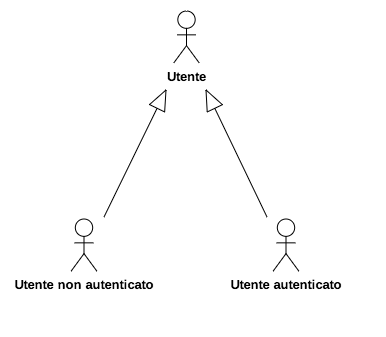
\includegraphics[scale=1]{../immagini/Actors.png}
\caption{Gerarchia attori}
\end{figure}

\newpage
\subsection{Sistema Quizzipedia}

\begin{figure}[h!]
\centering
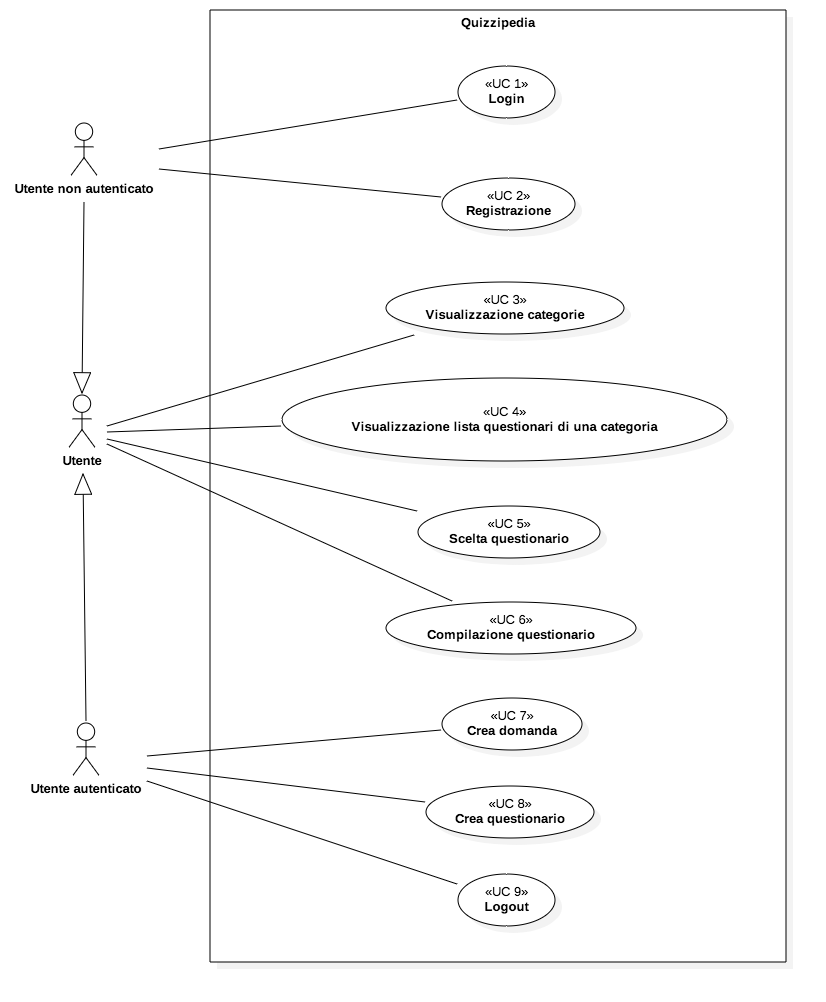
\includegraphics[scale=0.6]{../immagini/Main.png}
\caption{Sistema Quizzipedia}
\end{figure}
\ \\
\textbf{Attori:} \textit{utente non autenticato, utente autenticato}
\\ \\
\textbf{Descrizione:} caso d'uso generale che descrive le operazioni che i vari tipi di utenti possono effettuare all'interno del sistema.\\


\subsection{UC 1 - Login}

\begin{figure}[h!]
\centering
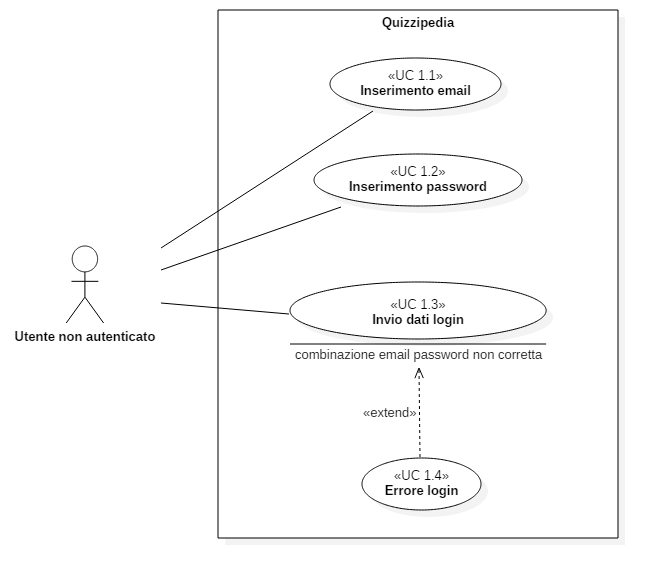
\includegraphics[scale=0.6]{../immagini/UC1.png}
\caption{Login}
\end{figure}
\ \\
\textbf{Attori:} \textit{utente non autenticato}
\\ \\
\textbf{Descrizione:} caso d'uso che descrive l'operazione di autenticazione al sistema. Comprende l'inserimento dei dati necessari, una procedura per il recupero della password e l'effettiva autenticazione.\\
\\
\textbf{Precondizioni:} il sistema può ricevere richieste di accesso da parte dell’utente non autenticato.\\
\\
\textbf{Postcondizioni:} l’utente che ora è autenticato.\\
\\
\textbf{Scenario:} l’utente inserisce i dati di accesso per effettuare il login al sistema (UC 1.1 e 1.2). Nel caso avesse dimenticato la password può accedere ad un form di recupero della stessa (UC 1.3). Se i dati inseriti sono corretti il sistema riconosce e autentica l'utente (UC 1.4) mentre se sono sbagliati viene visualizzato un messaggio di errore (UC 1.5).\\


\subsubsection{UC 1.1 - Inserimento email}

\textbf{Attori:} \textit{utente non autenticato}
\\ \\
\textbf{Descrizione:} caso d'uso che descrive l'inserimento della propria email da parte dell'utente.\\
\\
\textbf{Precondizioni:} il sistema permette l'inserimento di una email.\\
\\
\textbf{Postcondizioni:} l’utente ha inserito la propria email.\\
\\
\textbf{Scenario:} l’utente inserisce la propria email nell'apposito campo.\\


\subsubsection{UC 1.2 - Inserimento password}

\textbf{Attori:} \textit{utente non autenticato}
\\ \\
\textbf{Descrizione:} caso d'uso che descrive l'inserimento della propria password da parte dell'utente.\\
\\
\textbf{Precondizioni:} il sistema permette l'inserimento di una password.\\
\\
\textbf{Postcondizioni:} l’utente ha inserito la propria password.\\
\\
\textbf{Scenario:} l’utente inserisce la propria password nell'apposito campo.\\

\subsubsection{UC 1.3 - Invio dati login}

\textbf{Attori:} \textit{utente non autenticato}
\\ \\
\textbf{Descrizione:} caso d'uso che descrive l'autenticazione di un utente nel sistema.\\
\\
\textbf{Precondizioni:} l'utente ha inserito i propri dati e li ha inviati al sistema per l'autenticazione.\\
\\
\textbf{Postcondizioni:} l’utente è stato autenticato dal sistema.\\
\\
\textbf{Scenario:} l’utente invia i propri dati e il sistema lo autentica.\\
\\
\textbf{Extension points:} 
\begin{itemize}
	\item \textbf{Combinazione email password non corretta:} I dati inseriti e inviati al sistema non sono corretti, viene visualizzato un messaggio di errore (UC 1.5)
\end{itemize}


\subsubsection{UC 1.4 - Errore login}

\textbf{Attori:} \textit{utente non autenticato}
\\ \\
\textbf{Descrizione:} caso d'uso che descrive la visualizzazione del messaggio di errore sul tentativo di login.\\
\\
\textbf{Precondizioni:} l'utente ha inserito i propri dati e li ha inviati al sistema per l'autenticazione. La combinazione di username e password non è corretta.\\
\\
\textbf{Postcondizioni:} l’utente visualizza un messaggio di errore sul tentativo di login.\\
\\
\textbf{Scenario:} viene visualizzato un messaggio di errore sul tentativo di login.\\


\subsection{UC 2 - Registrazione}

\begin{figure}[h!]
\centering
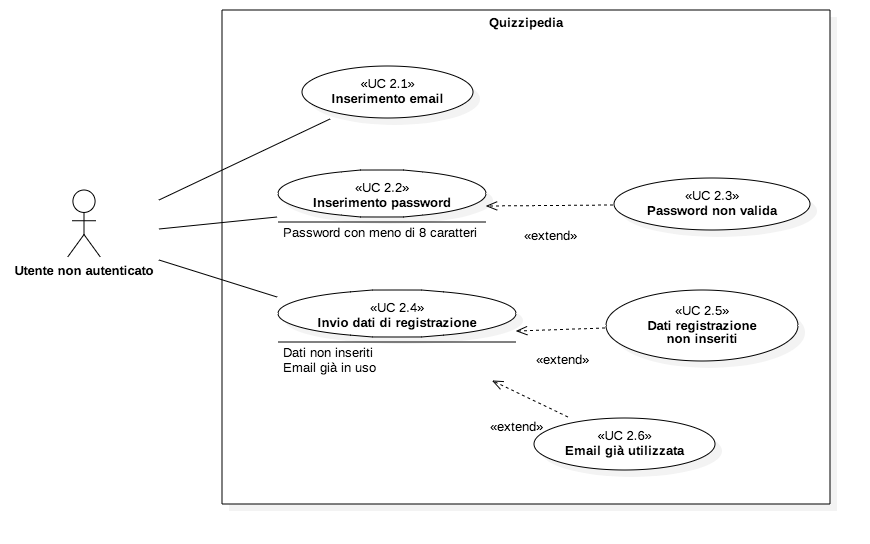
\includegraphics[scale=0.6]{../immagini/UC2.png}
\caption{Registrazione}
\end{figure}
\ \\
\textbf{Attori:} \textit{utente non autenticato}
\\ \\
\textbf{Descrizione:} caso d'uso che descrive l'operazione di registrazione al sistema. Comprende l'inserimento dei dati necessari, l'effettiva registrazione e l'autenticazione.\\
\\
\textbf{Precondizioni:} il sistema può registrare un nuovo utente.\\
\\
\textbf{Postcondizioni:} l’utente che ora è registrato e autenticato.\\
\\
\textbf{Scenario:} l’utente inserisce i dati di registrazione per effettuare il login al sistema (UC 2.1 e 2.2). Nel caso la password non abbia almeno 8 caratteri viene visualizzato un messaggio che avvisa l'utente che non è valida (UC 2.3). Se i dati inseriti sono corretti il sistema registra e autentica l'utente (UC 2.4). Se invece non sono stati inseriti alcuni campi viene visualizzato un messaggio di errore (UC 2.5). Nel caso in cui la email inserita sia già utilizzata da un altro utente viene visualizzato un messaggio di errore (UC 2.6).\\


\subsubsection{UC 2.1 - Inserimento email}

\textbf{Attori:} \textit{utente non autenticato}
\\ \\
\textbf{Descrizione:} caso d'uso che descrive l'inserimento della propria email da parte dell'utente.\\
\\
\textbf{Precondizioni:} il sistema permette l'inserimento di una email.\\
\\
\textbf{Postcondizioni:} l’utente ha inserito la propria email.\\
\\
\textbf{Scenario:} l’utente inserisce la propria email nell'apposito campo.\\


\subsubsection{UC 2.2 - Inserimento password}

\textbf{Attori:} \textit{utente non autenticato}
\\ \\
\textbf{Descrizione:} caso d'uso che descrive l'inserimento della propria password da parte dell'utente.\\
\\
\textbf{Precondizioni:} il sistema permette l'inserimento di una password.\\
\\
\textbf{Postcondizioni:} l’utente ha inserito la propria password.\\
\\
\textbf{Scenario:} l’utente inserisce la propria password nell'apposito campo.\\
\\
\textbf{Extension points:} 
\begin{itemize}
	\item \textbf{Password non valida:} La password non è valida in quanto è formata da meno di 8 caratteri, viene visualizzato un messaggio di errore (UC 2.3)
\end{itemize}


\subsubsection{UC 2.3 - Password non valida}

\textbf{Attori:} \textit{utente non autenticato}
\\ \\
\textbf{Descrizione:} caso d'uso che descrive la visualizzazione del messaggio di errore relativo all'invalidità della password.\\
\\
\textbf{Precondizioni:} l'utente ha inserito la propria password. La password non è valida, ovvero ha meno di 8 caratteri.\\
\\
\textbf{Postcondizioni:} l’utente visualizza un messaggio di errore relativo all'invalidità della password.\\
\\
\textbf{Scenario:} viene visualizzato un messaggio di errore relativo all'invalidità della password.\\


\subsubsection{UC 2.4 - Invio dati registrazione}

\textbf{Attori:} \textit{utente non autenticato}
\\ \\
\textbf{Descrizione:} caso d'uso che descrive la registrazione e l'autenticazione di un utente nel sistema.\\
\\
\textbf{Precondizioni:} l'utente ha inserito i propri dati e li ha inviati al sistema per la registrazione.\\
\\
\textbf{Postcondizioni:} l’utente è stato registrato e autenticato dal sistema.\\
\\
\textbf{Scenario:} l’utente invia i propri dati e il sistema lo registra come nuovo utente e lo autentica.\\
\\
\textbf{Extension points:} 
\begin{itemize}
	\item \textbf{Dati non inseriti:} alcuni dati richiesti non sono stati inseriti, viene visualizzato un messaggio di errore (UC 2.5)
	\item \textbf{email già in uso:} l'email inserita è già stata registrata da un utente, viene visualizzato un messaggio di errore (UC 2.6)
\end{itemize}


\subsubsection{UC 2.5 - Dati registrazione non inseriti}

\textbf{Attori:} \textit{utente non autenticato}
\\ \\
\textbf{Descrizione:} caso d'uso che descrive la visualizzazione del messaggio di errore relativo alla mancanza di dati necessari alla registrazione.\\
\\
\textbf{Precondizioni:} l'utente ha inserito i propri dati e li ha inviati al sistema per la registrazione. Almeno un dato necessario non è stato inserito.\\
\\
\textbf{Postcondizioni:} l’utente visualizza un messaggio di errore relativo alla mancanza di dati necessari alla registrazione.\\
\\
\textbf{Scenario:} viene visualizzato un messaggio di errore relativo alla mancanza di dati necessari alla registrazione.\\


\subsubsection{UC 2.6 - Email già utilizzata}

\textbf{Attori:} \textit{utente non autenticato}
\\ \\
\textbf{Descrizione:} caso d'uso che descrive la visualizzazione del messaggio di errore relativo alla email già registrata alla registrazione.\\
\\
\textbf{Precondizioni:} l'utente ha inserito i propri dati e li ha inviati al sistema per la registrazione. L'email inserita è già stata registrata.\\
\\
\textbf{Postcondizioni:} l’utente visualizza un messaggio di errore relativo alla email già registrata alla registrazione.\\
\\
\textbf{Scenario:} viene visualizzato un messaggio di errore relativo alla email già registrata alla registrazione.\\


\subsection{UC 3 - Visualizzazione categorie}

\begin{figure}[h!]
\centering
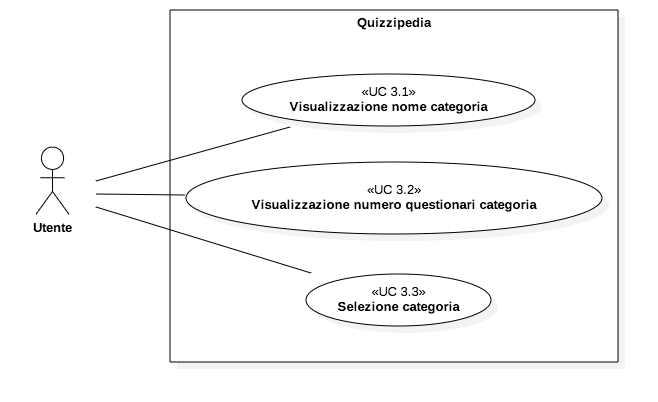
\includegraphics[scale=0.6]{../immagini/UC3.png}
\caption{Visualizzazione categorie}
\end{figure}
\ \\
\textbf{Attori:} \textit{utente}
\\ \\
\textbf{Descrizione:} caso d'uso che descrive la visualizzazione delle categorie di questionari. Per ogni categoria vengono visualizzati il nome e il numero di questionari relativi.\\
\\
\textbf{Precondizioni:} il sistema può accedere alla lista categorie.\\
\\
\textbf{Postcondizioni:} l’utente visualizza la lista delle categorie presenti.\\
\\
\textbf{Scenario:} l’utente accede alla sezione "Categorie". Per ogni categoria vengono visualizzati il nome (UC 3.1) e il numero di questionari relativi (UC 3.2). L'utente può selezionare una categoria (UC 3.3)\\


\subsubsection{UC 3.1 - Visualizzazione nome categoria}

\textbf{Attori:} \textit{utente}
\\ \\
\textbf{Descrizione:} caso d'uso che descrive la visualizzazione dei nomi delle categorie.\\
\\
\textbf{Precondizioni:} L'utente è nella sezione "categorie".\\
\\
\textbf{Postcondizioni:} il sistema visualizza i nomi delle categorie.\\
\\
\textbf{Scenario:} l’utente visualizza i nomi delle categorie.\\


\subsubsection{UC 3.2 - Visualizzazione numero questionari categoria}

\textbf{Attori:} \textit{utente}
\\ \\
\textbf{Descrizione:} caso d'uso che descrive la visualizzazione del numero di questionari delle categorie.\\
\\
\textbf{Precondizioni:} L'utente è nella sezione "categorie".\\
\\
\textbf{Postcondizioni:} il sistema visualizza il numero di questionari delle categorie.\\
\\
\textbf{Scenario:} l’utente visualizza il numero di questionari delle categorie.\\


\subsubsection{UC 3.3 - Selezione categoria}

\textbf{Attori:} \textit{utente}
\\ \\
\textbf{Descrizione:} caso d'uso che descrive la selezione di una categoria.\\
\\
\textbf{Precondizioni:} L'utente è nella sezione "categorie".\\
\\
\textbf{Postcondizioni:} la categoria è stata selezionata e viene visualizzata la lista dei questionari relativi.\\
\\
\textbf{Scenario:} l’utente seleziona una categoria e il sistema visualizza la lista dei questionari relativi.\\


\newpage
\subsection{UC 4 - Visualizzazione lista questionari categoria}

\begin{figure}[h!]
\centering
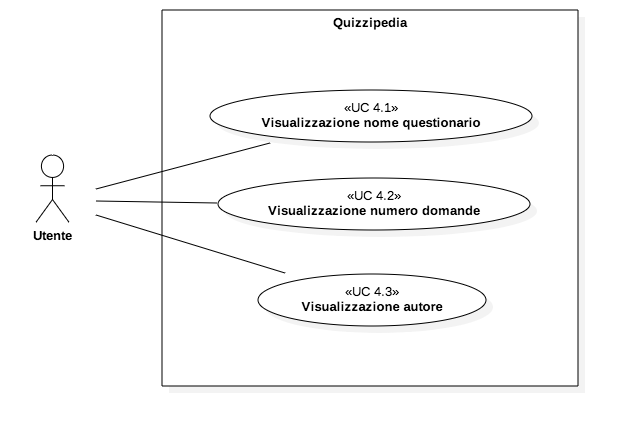
\includegraphics[scale=0.6]{../immagini/UC4.png}
\caption{Visualizzazione lista questionari categoria}
\end{figure}
\ \\
\textbf{Attori:} \textit{utente}
\\ \\
\textbf{Descrizione:} caso d'uso che descrive la visualizzazione della lista dei questionari di una categoria. Per ogni questionario vengono visualizzati il nome, il numero di domande e l'autore.\\
\\
\textbf{Precondizioni:} l'utente ha selezionato una categoria.\\
\\
\textbf{Postcondizioni:} l’utente visualizza la lista dei questionari della categoria selezionata.\\
\\
\textbf{Scenario:} l’utente seleziona una categoria e visualizza i questionari relativi. Per ogni questionario vengono visualizzati il nome (UC 4.1), il numero di domande (UC 4.2), l'autore (UC 4.3) e la data di creazione (UC 4.4).\\


\subsubsection{UC 4.1 - Visualizzazione nome questionario}

\textbf{Attori:} \textit{utente}
\\ \\
\textbf{Descrizione:} caso d'uso che descrive la visualizzazione dei nomi dei questionari.\\
\\
\textbf{Precondizioni:} L'utente visualizza la lista dei questionari della categoria selezionata.\\
\\
\textbf{Postcondizioni:} il sistema visualizza i nomi dei questionari.\\
\\
\textbf{Scenario:} l’utente visualizza i nomi dei questionari.\\


\subsubsection{UC 4.2 - Visualizzazione numero domande}

\textbf{Attori:} \textit{utente}
\\ \\
\textbf{Descrizione:} caso d'uso che descrive la visualizzazione del numero di domande dei questionari.\\
\\
\textbf{Precondizioni:} l'utente visualizza la lista dei questionari della categoria selezionata.\\
\\
\textbf{Postcondizioni:} il sistema visualizza il numero di domande dei questionari.\\
\\
\textbf{Scenario:} l’utente visualizza il numero di domande dei questionari.\\


\subsubsection{UC 4.3 - Visualizzazione autore}

\textbf{Attori:} \textit{utente}
\\ \\
\textbf{Descrizione:} caso d'uso che descrive la visualizzazione degli autori dei questionari.\\
\\
\textbf{Precondizioni:} l'utente visualizza la lista dei questionari della categoria selezionata.\\
\\
\textbf{Postcondizioni:} il sistema visualizza gli autori dei questionari.\\
\\
\textbf{Scenario:} l’utente visualizza gli autori dei questionari.\\


\subsubsection{UC 4.4 - Visualizzazione autore}

\textbf{Attori:} \textit{utente}
\\ \\
\textbf{Descrizione:} caso d'uso che descrive la visualizzazione delle date di creazione dei questionari.\\
\\
\textbf{Precondizioni:} l'utente visualizza la lista dei questionari della categoria selezionata.\\
\\
\textbf{Postcondizioni:} il sistema visualizza le date di creazione dei questionari.\\
\\
\textbf{Scenario:} l’utente visualizza le date di creazione dei questionari.\\


\subsection{UC 5 - Scelta questionario}

\textbf{Attori:} \textit{utente}
\\ \\
\textbf{Descrizione:} caso d'uso che descrive la scelta di un questionario.\\
\\
\textbf{Precondizioni:} il sistema permette la selezione di questionari.\\
\\
\textbf{Postcondizioni:} l’utente ha selezionato un questionario e può procedere con la compilazione.\\
\\
\textbf{Scenario:} l’utente seleziona un questionario. Il sistema entra in modalità compilazione del questionario.\\


\subsection{UC 6 - Compilazione questionario}

\begin{figure}[h!]
\centering
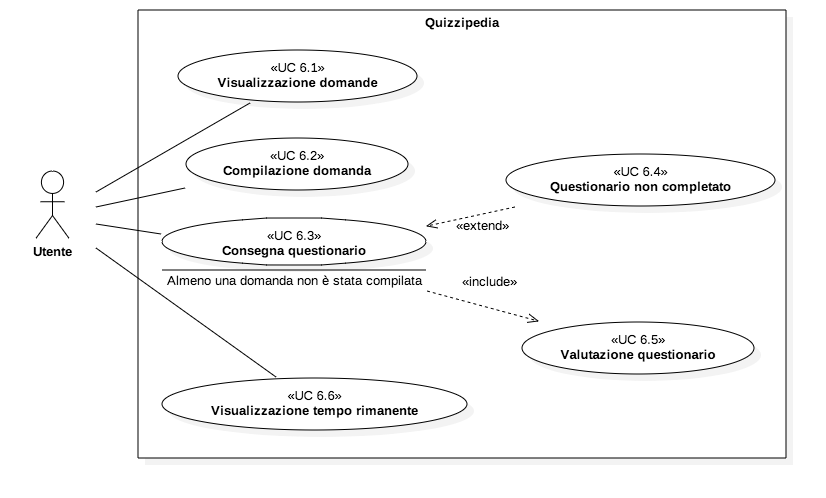
\includegraphics[scale=0.5]{../immagini/UC6.png}
\caption{Compilazione questionario}
\end{figure}
\ \\
\textbf{Attori:} \textit{utente}
\\ \\
\textbf{Descrizione:} caso d'uso che descrive la compilazione di un questionario. Comprende la visualizzazione e compilazione delle domande, la consegna e la valutazione del questionario.\\
\\
\textbf{Precondizioni:} l'utente può compilare un questionario.\\
\\
\textbf{Postcondizioni:} l’utente ha compilato un questionario e ne vede la valutazione.\\
\\
\textbf{Scenario:} l’utente compila il questionario. Questo comprende la visualizzazione e la compilazione delle domande (UC 6.1, UC 6.2), la navigazione tra esse (UC 6.6, UC 6.7) e la consegna (UC 6.3). La consegna viene eseguita in automatico allo scadere del tempo di compilazione. In caso alla consegna ci siano domande non compilate e il tempo non sia scaduto viene visualizzato un messaggio di errore (UC 6.4). Dopo la consegna avviene la valutazione del questionario e la visualizzazione dei risultati (UC 6.5). Durante la compilazione viene visualizzato il tempo rimanente (UC 6.6).\\


\subsubsection{UC 6.1 - Visualizzazione domanda}

\begin{figure}[h!]
\centering
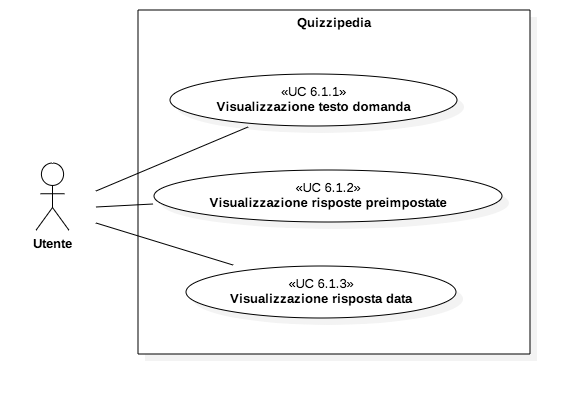
\includegraphics[scale=0.6]{../immagini/UC6_1.png}
\caption{Visualizzazione domanda}
\end{figure}
\ \\
\textbf{Attori:} \textit{utente}
\\ \\
\textbf{Descrizione:} caso d'uso che descrive la visualizzazione della domanda attuale di un questionario.\\
\\
\textbf{Precondizioni:} l'utente sta compilando un questionario.\\
\\
\textbf{Postcondizioni:} il sistema visualizza la domanda attuale del questionario.\\
\\
\textbf{Scenario:} l’utente sta svolgendo un questionario e gli viene presentata a video una domanda al quale deve rispondere.\\


\subsubsubsection{UC 6.1.1 - Visualizzazione testo domanda}

\textbf{Attori:} \textit{utente}
\\ \\
\textbf{Descrizione:} caso d'uso che descrive la visualizzazione del testo della domanda.\\
\\
\textbf{Precondizioni:} l'utente si appresta a rispondere ad una domanda.\\
\\
\textbf{Postcondizioni:} il sistema visualizza il testo della domanda.\\
\\
\textbf{Scenario:} l’utente visualizza il testo della domanda.\\


\subsubsubsection{UC 6.1.2 - Visualizzazione risposte preimpostate}

\textbf{Attori:} \textit{utente}
\\ \\
\textbf{Descrizione:} caso d'uso che descrive la visualizzazione su schermo delle risposte (immediatamente sotto il testo della domanda).\\
\\
\textbf{Precondizioni:} l'utente visualizza una domanda. La domanda ha delle risposte preimpostate di qualsiasi tipo tra le quali l'utente dovrà scegliere.\\
\\
\textbf{Postcondizioni:} il sistema visualizza le risposte della domanda su schermo (immediatamente sotto il testo della domanda).\\
\\
\textbf{Scenario:} l’utente visualizza le risposte nel formato relativo alla domanda (tra queste risposte ne sceglierà quella che ritiene corretta)\\


\subsubsubsection{UC 6.1.3 - Visualizzazione risposta data}

\textbf{Attori:} \textit{utente}
\\ \\
\textbf{Descrizione:} caso d'uso che descrive la visualizzazione della risposta data.\\
\\
\textbf{Precondizioni:} l'utente ha risposto ad una domanda.\\
\\
\textbf{Postcondizioni:} il sistema evidenzia la risposta data.\\
\\
\textbf{Scenario:} la risposta data dall'utente viene evidenziata su schermo ed è facilmente distinguibile dall'utente.\\


\newpage
\subsubsection{UC 6.2 - Compilazione domanda}

\begin{figure}[h!]
\centering
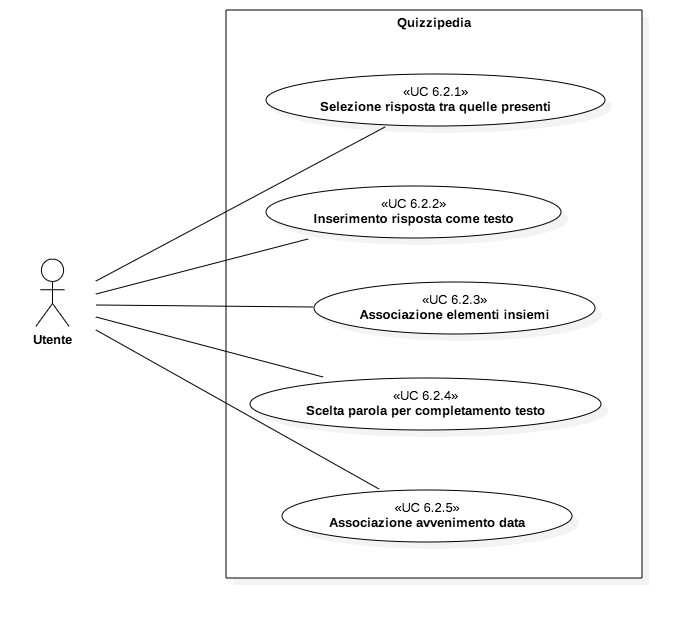
\includegraphics[scale=0.6]{../immagini/UC6_2.png}
\caption{Compilazione domanda}
\end{figure}
\ \\
\textbf{Attori:} \textit{utente}
\\ \\
\textbf{Descrizione:} caso d'uso che descrive la compilazione di una domanda.\\
\\
\textbf{Precondizioni:} l'utente visualizza una domanda.\\
\\
\textbf{Postcondizioni:} l'utente ha compilato una domanda.\\
\\
\textbf{Scenario:} l’utente sta visualizzando una domanda e la compila.\\


\subsubsubsection{UC 6.2.1 - Selezione risposta tra le presenti}

\textbf{Attori:} \textit{utente}
\\ \\
\textbf{Descrizione:} caso d'uso che descrive la selezione di una delle risposte preimpostate.\\
\\
\textbf{Precondizioni:} l'utente visualizza una domanda con risposte preimpostate.\\
\\
\textbf{Postcondizioni:} l'utente ha selezionato una risposta.\\
\\
\textbf{Scenario:} l’utente seleziona una delle risposte preimpostate.\\


\subsubsubsection{UC 6.2.2 - Inserimento risposta come testo}

\textbf{Attori:} \textit{utente}
\\ \\
\textbf{Descrizione:} caso d'uso che descrive l'inserimento della risposta.\\
\\
\textbf{Precondizioni:} l'utente visualizza una domanda a risposta testuale. Il sistema permette l'inserimento della risposta.\\
\\
\textbf{Postcondizioni:} l'utente ha inserito una risposta.\\
\\
\textbf{Scenario:} l’utente inserisce una risposta nel campo apposito.\\


\subsubsubsection{UC 6.2.3 - Associazione tra elementi di due insiemi}

\textbf{Attori:} \textit{utente}
\\ \\
\textbf{Descrizione:} caso d'uso che descrive l'associazione di elementi di due insiemi.\\
\\
\textbf{Precondizioni:} l'utente visualizza una domanda di associazione tra insiemi.\\
\\
\textbf{Postcondizioni:} l'utente ha associato due elementi.\\
\\
\textbf{Scenario:} l’utente associa due elementi di due insiemi.\\


\subsubsubsection{UC 6.2.4 - Scelta di una parola per il completamento del testo}

\textbf{Attori:} \textit{utente}
\\ \\
\textbf{Descrizione:} caso d'uso che descrive la scelta di una parola tra le presenti per il completamento del testo.\\
\\
\textbf{Precondizioni:} l'utente visualizza una domanda in cui si deve completare un testo utilizzando le parole fornite.\\
\\
\textbf{Postcondizioni:} l'utente ha completato il testo o parte di esso utilizzando una parola tra quelle fornite.\\
\\
\textbf{Scenario:} l’utente completa il testo o parte di esso inserendo una parola tra quelle fornite.\\


\subsubsubsection{UC 6.2.5 - Associazione tra avvenimento e data}

\textbf{Attori:} \textit{utente}
\\ \\
\textbf{Descrizione:} caso d'uso che descrive l'associazione tra un avvenimento e una data.\\
\\
\textbf{Precondizioni:} l'utente visualizza una domanda di tipo timeline.\\
\\
\textbf{Postcondizioni:} l'utente ha associato un avvenimento ad una data.\\
\\
\textbf{Scenario:} l’utente associa un avvenimento ad una data sulla timeline.\\


\subsubsection{UC 6.3 - Consegna questionario}

\textbf{Attori:} \textit{utente}
\\ \\
\textbf{Descrizione:} caso d'uso che descrive la consegna di un questionario. Viene eseguito in automatico dal sistema quando si esaurisce il tempo di compilazione.\\
\\
\textbf{Precondizioni:} l'utente ha compilato un questionario.\\
\\
\textbf{Postcondizioni:} l’utente ha consegnato il questionario e ne ha ricevuto una valutazione.\\
\\
\textbf{Scenario:} l’utente consegna il questionario. Il sistema lo valuta e visualizza i risultati (UC 6.5).\\
\\
\textbf{Extension points:} 
\begin{itemize}
	\item \textbf{Domanda non compilata:} almeno una domanda non  è stata compilata e il tempo non è scaduto, viene visualizzato un messaggio di errore (UC 6.4)
\end{itemize}


\subsubsubsection{UC 6.4 - Questionario non completato}

\textbf{Attori:} \textit{utente}
\\ \\
\textbf{Descrizione:} caso d'uso che descrive la visualizzazione del messaggio di errore relativo alla consegna di un questionario non completo.\\
\\
\textbf{Precondizioni:} l'utente ha consegnato il questionario incompleto e il tempo non è scaduto.\\
\\
\textbf{Postcondizioni:} l'utente visualizza il messaggio di errore relativo alla consegna di un questionario non completo.\\
\\
\textbf{Scenario:} l’utente consegna un questionario incompleto e visualizza il messaggio di errore relativo.\\


\subsubsection{UC 6.5 - Visualizzazione risultati}

\begin{figure}[h!]
\centering
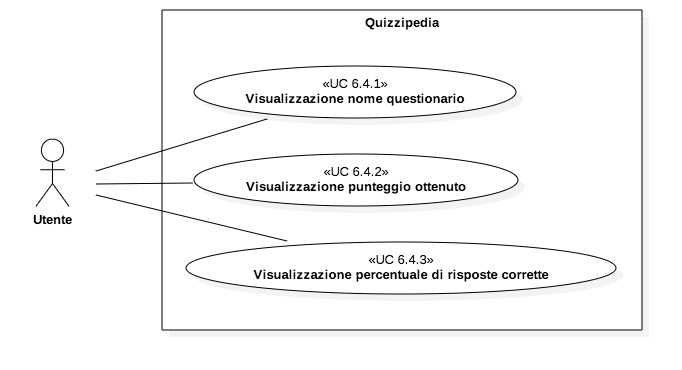
\includegraphics[scale=0.6]{../immagini/UC6_5.png}
\caption{Visualizzazione risultati}
\end{figure}
\ \\
\textbf{Attori:} \textit{utente}
\\ \\
\textbf{Descrizione:} caso d'uso che descrive la visualizzazione della valutazione di un questionario consegnato.\\
\\
\textbf{Precondizioni:} l'utente ha compilato e consegnato un questionario.\\
\\
\textbf{Postcondizioni:} l'utente visualizza la valutazione del questionario.\\
\\
\textbf{Scenario:} il sistema valuta il questionario completato dall'utente e visualizza i risultati della correzione su schermo (l'utente non compie nessuna particolare azione, semplicemente attende qualche secondo dopo la consegna del questionario)\\


\subsubsubsection{UC 6.5.1 - Visualizzazione nome questionario}

\textbf{Attori:} \textit{utente}
\\ \\
\textbf{Descrizione:} caso d'uso che descrive la visualizzazione del nome del questionario valutato.\\
\\
\textbf{Precondizioni:} l'utente ha consegnato un questionario che è stato valutato dal sistema.\\
\\
\textbf{Postcondizioni:} il sistema visualizza il nome del questionario valutato.\\
\\
\textbf{Scenario:} l’utente visualizza il nome del questionario valutato.\\


\subsubsubsection{UC 6.5.2 - Visualizzazione punteggio ottenuto}

\textbf{Attori:} \textit{utente}
\\ \\
\textbf{Descrizione:} caso d'uso che descrive la visualizzazione del punteggio ottenuto nel questionario valutato.\\
\\
\textbf{Precondizioni:} l'utente ha consegnato un questionario che è stato valutato dal sistema.\\
\\
\textbf{Postcondizioni:} il sistema visualizza il punteggio ottenuto nel questionario valutato.\\
\\
\textbf{Scenario:} l’utente visualizza il punteggio ottenuto nel questionario valutato.\\


\subsubsubsection{UC 6.5.3 - Visualizzazione percentuale risposte corrette}

\textbf{Attori:} \textit{utente}
\\ \\
\textbf{Descrizione:} caso d'uso che descrive la visualizzazione della percentuale risposte corrette nel questionario valutato.\\
\\
\textbf{Precondizioni:} l'utente ha consegnato un questionario che è stato valutato dal sistema.\\
\\
\textbf{Postcondizioni:} il sistema visualizza la percentuale risposte corrette nel questionario valutato.\\
\\
\textbf{Scenario:} l’utente visualizza la percentuale risposte corrette nel questionario valutato.\\


\subsubsection{UC 6.6 - Visualizzazione tempo rimanente}

\textbf{Attori:} \textit{utente}
\\ \\
\textbf{Descrizione:} caso d'uso che descrive la visualizzazione del tempo rimanente per la compilazione del questionario.\\
\\
\textbf{Precondizioni:} l'utente sta compilando un questionario.\\
\\
\textbf{Postcondizioni:} l'utente visualizza il tempo rimanente per la compilazione del questionario.\\
\\
\textbf{Scenario:} il sistema visualizza il tempo rimanente per la compilazione.\\


\subsubsection{UC 6.7 - Domanda successiva}

\textbf{Attori:} \textit{utente}
\\ \\
\textbf{Descrizione:} caso d'uso che descrive il passaggio alla domanda successiva.\\
\\
\textbf{Precondizioni:} l'utente sta compilando un questionario. La domanda attuale non è l'ultima.\\
\\
\textbf{Postcondizioni:} l'utente visualizza la domanda successiva a quella appena visualizzata.\\
\\
\textbf{Scenario:} il sistema visualizza la domanda successiva.\\


\subsubsection{UC 6.8 - Domanda precedente}

\textbf{Attori:} \textit{utente}
\\ \\
\textbf{Descrizione:} caso d'uso che descrive il passaggio alla domanda precedente.\\
\\
\textbf{Precondizioni:} l'utente sta compilando un questionario. La domanda attuale non è la prima.\\
\\
\textbf{Postcondizioni:} l'utente visualizza la domanda precedente a quella appena visualizzata.\\
\\
\textbf{Scenario:} il sistema visualizza la domanda precedente.\\


\subsection{UC 7 - Gestione domande}

\begin{figure}[h!]
\centering
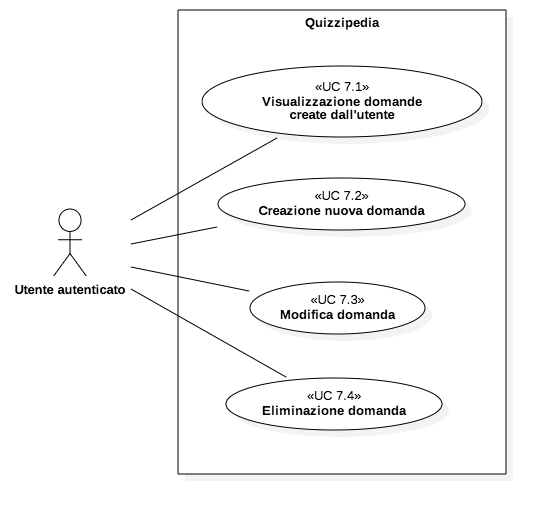
\includegraphics[scale=0.6]{../immagini/UC7.png}
\caption{Gestione domande}
\end{figure}
\ \\
\textbf{Attori:} \textit{utente autenticato}
\\ \\
\textbf{Descrizione:} caso d'uso che descrive la gestione delle domande che un utente ha creato o vuole creare.\\
\\
\textbf{Precondizioni:} l'utente può gestire domande.\\
\\
\textbf{Postcondizioni:} l’utente ha gestito le proprie domande.\\
\\
\textbf{Scenario:} l’utente visualizza le proprie domande (UC 7.1). Può crearne una nuova (UC 7.2), modificarne una esistente (UC 7.3) o eliminarne una (UC 7.4).\\


\subsubsection{UC 7.1 - Visualizzazione domande create dall'utente}

\begin{figure}[h!]
\centering
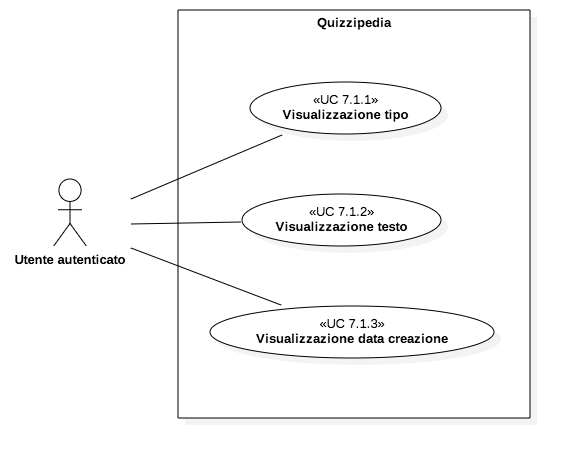
\includegraphics[scale=0.6]{../immagini/UC7_1.png}
\caption{Visualizzazione domande create dall'utente}
\end{figure}
\ \\
\textbf{Attori:} \textit{utente autenticato}
\\ \\
\textbf{Descrizione:} caso d'uso che descrive la visualizzazione delle domande create dall'utente.\\
\\
\textbf{Precondizioni:} l'utente è entrato nella sezione di gestione delle proprie domande.\\
\\
\textbf{Postcondizioni:} l’utente visualizza le proprie domande.\\
\\
\textbf{Scenario:} l’utente è entrato nella sezione di gestione delle proprie domande e ne visualizza il tipo (UC 7.1.1), il testo (UC 7.1.2) e la data di creazione (UC 7.1.3).\\


\subsubsubsection{UC 7.1.1 - Visualizzazione tipo}

\textbf{Attori:} \textit{utente autenticato}
\\ \\
\textbf{Descrizione:} caso d'uso che descrive la visualizzazione del tipo delle domande.\\
\\
\textbf{Precondizioni:} l'utente visualizza le domande da lui create.\\
\\
\textbf{Postcondizioni:} il sistema visualizza il tipo delle domande.\\
\\
\textbf{Scenario:} l’utente visualizza il tipo delle domande.\\


\subsubsubsection{UC 7.1.2 - Visualizzazione testo}

\textbf{Attori:} \textit{utente autenticato}
\\ \\
\textbf{Descrizione:} caso d'uso che descrive la visualizzazione del testo delle domande.\\
\\
\textbf{Precondizioni:} l'utente visualizza le domande da lui create.\\
\\
\textbf{Postcondizioni:} il sistema visualizza il testo delle domande.\\
\\
\textbf{Scenario:} l’utente visualizza il testo delle domande.\\


\subsubsubsection{UC 7.1.3 - Visualizzazione data creazione}

\textbf{Attori:} \textit{utente autenticato}
\\ \\
\textbf{Descrizione:} caso d'uso che descrive la visualizzazione della data di creazione delle domande.\\
\\
\textbf{Precondizioni:} l'utente visualizza le domande da lui create.\\
\\
\textbf{Postcondizioni:} il sistema visualizza la data di creazione delle domande.\\
\\
\textbf{Scenario:} l’utente visualizza la data di creazione delle domande.\\


\newpage
\subsubsection{UC 7.2 - Creazione nuova domanda}

\begin{figure}[h!]
\centering
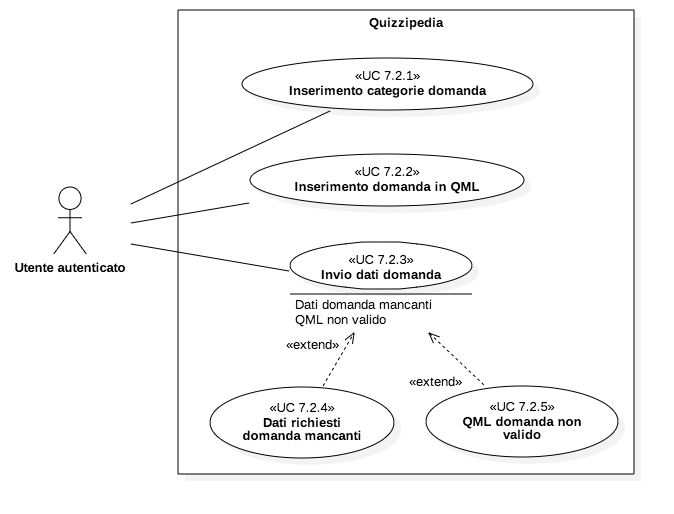
\includegraphics[scale=0.6]{../immagini/UC7_2.png}
\caption{Creazione domanda}
\end{figure}
\ \\
\textbf{Attori:} \textit{utente autenticato}
\\ \\
\textbf{Descrizione:} caso d'uso che descrive la creazione di una nuova domanda.\\
\\
\textbf{Precondizioni:} l'utente può creare una domanda.\\
\\
\textbf{Postcondizioni:} l’utente ha creato una nuova domanda.\\
\\
\textbf{Scenario:} l’utente inserisce i dati della domanda (UC 7.2.1, UC 7.2.2) e li invia al sistema che memorizza la nuova domanda (UC 7.2.3). Se all'invio alcuni dati essenziali mancano o il codice QML inserito non è valido viene visualizzato un messaggio di errore (UC 7.2.4, UC 7.2.5). Alternativamente in qualsiasi momento l'utente può annullare la creazione e tornare indietro.\\


\subsubsubsection{UC 7.2.1 - Inserimento categorie domanda}

\textbf{Attori:} \textit{utente autenticato}
\\ \\
\textbf{Descrizione:} caso d'uso che descrive l'inserimento delle categorie della domanda.\\
\\
\textbf{Precondizioni:} il sistema permette l'inserimento di una o più categorie.\\
\\
\textbf{Postcondizioni:} l’utente ha inserito almeno una categoria.\\
\\
\textbf{Scenario:} l’utente inserisce una o più categorie nell'apposito campo.\\


\subsubsubsection{UC 7.2.2 - Inserimento QML domanda}

\textbf{Attori:} \textit{utente autenticato}
\\ \\
\textbf{Descrizione:} caso d'uso che descrive l'inserimento del codice QML che descrive la domanda.\\
\\
\textbf{Precondizioni:} il sistema permette l'inserimento di codice QML.\\
\\
\textbf{Postcondizioni:} l’utente ha inserito il codice QML che descrive la domanda.\\
\\
\textbf{Scenario:} l’utente inserisce il codice QML che descrive la domanda nell'apposita area di testo.\\


\subsubsubsection{UC 7.2.3 - Invio dati domanda}

\textbf{Attori:} \textit{utente autenticato}
\\ \\
\textbf{Descrizione:} caso d'uso che descrive l'invio dei dati della nuova domanda.\\
\\
\textbf{Precondizioni:} l'utente ha inserito i dati della domanda.\\
\\
\textbf{Postcondizioni:} l’utente ha inviato i dati della domanda e il sistema l'ha memorizzata nel database.\\
\\
\textbf{Scenario:} l’utente invia i dati della domanda. Il sistema memorizza nel database la nuova domanda.\\
\\
\textbf{Extension points:} 
\begin{itemize}
	\item \textbf{Dati domanda mancanti:} almeno un dato richiesto non è stato inserito dall'utente, viene visualizzato un messaggio di errore (UC 7.2.4)
	\item \textbf{QML non valido:} il codice QML inserito dall'utente non rispetta la sintassi del QML, viene visualizzato un messaggio di errore (UC 7.2.5)
\end{itemize}


\subsubsubsection{UC 7.2.4 - Dati richiesti domanda mancanti}

\textbf{Attori:} \textit{utente autenticato}
\\ \\
\textbf{Descrizione:} caso d'uso che descrive la visualizzazione del messaggio di errore relativo alla mancanza di dati necessari.\\
\\
\textbf{Precondizioni:} l'utente ha confermato la creazione della domanda. Almeno un dato necessario alla creazione non è stato inserito.\\
\\
\textbf{Postcondizioni:} l’utente visualizza il messaggio di errore relativo alla mancanza di dati necessari.\\
\\
\textbf{Scenario:} l'utente conferma la creazione di una domanda senza inserire almeno una informazione necessaria e visualizza il relativo messaggio di errore.\\


\subsubsubsection{UC 7.2.5 - QML domanda non valido}

\textbf{Attori:} \textit{utente autenticato}
\\ \\
\textbf{Descrizione:} caso d'uso che descrive la visualizzazione del messaggio di errore per il codice QML non valido inserito.\\
\\
\textbf{Precondizioni:} l'utente ha confermato la creazione della domanda. Il codice QML inserito non è valido.\\
\\
\textbf{Postcondizioni:} l’utente visualizza il messaggio di errore per il codice QML non valido inserito.\\
\\
\textbf{Scenario:} l'utente conferma la creazione di una domanda inserendo un codice QML invalido e visualizza il relativo messaggio di errore.\\


\newpage
\subsubsection{UC 7.3 - Modifica domanda}

\begin{figure}[h!]
\centering
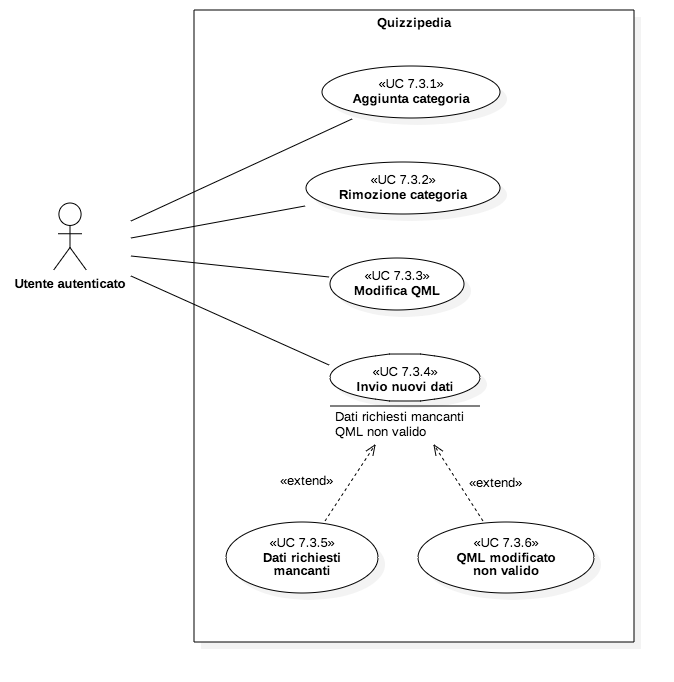
\includegraphics[scale=0.6]{../immagini/UC7_3.png}
\caption{Modifica domanda}
\end{figure}
\ \\
\textbf{Attori:} \textit{utente autenticato}
\\ \\
\textbf{Descrizione:} caso d'uso che descrive la modifica di una domanda creata dall'utente.\\
\\
\textbf{Precondizioni:} l'utente è entrato nella sezione di gestione delle proprie domande.\\
\\
\textbf{Postcondizioni:} l’utente ha modificato una propria domanda.\\
\\
\textbf{Scenario:} l’utente modifica una propria domanda aggiungendo o rimuovendo categorie (UC 7.3.1, UC 7.3.2), modificandone il codice QML che le descrive (UC 7.3.3). Al termine delle modifiche invia i nuovi dati al sistema che modifica effettivamente la domanda (UC 7.3.4). Nel caso in cui alcuni dati manchino o il nuovo codice QML non sia valido viene visualizzato un messaggio di errore (UC 7.3.5, UC 7.3.6).\\


\subsubsubsection{UC 7.3.1 - Aggiunta categoria}

\textbf{Attori:} \textit{utente autenticato}
\\ \\
\textbf{Descrizione:} caso d'uso che descrive l'aggiunta di una categoria che la domanda riguarda.\\
\\
\textbf{Precondizioni:} l'utente sta modificando una propria domanda.\\
\\
\textbf{Postcondizioni:} l’utente ha aggiunto una categoria alla domanda.\\
\\
\textbf{Scenario:} l’utente aggiunge una categoria alla domanda.\\


\subsubsubsection{UC 7.3.2 - Rimozione categoria}

\textbf{Attori:} \textit{utente autenticato}
\\ \\
\textbf{Descrizione:} caso d'uso che descrive la rimozione di una categoria dalla domanda.\\
\\
\textbf{Precondizioni:} l'utente sta modificando una propria domanda.\\
\\
\textbf{Postcondizioni:} l’utente ha rimosso una categoria dalla domanda.\\
\\
\textbf{Scenario:} l’utente rimuove una categoria dalla domanda.\\


\subsubsubsection{UC 7.3.3 - Modifica QML domanda}

\textbf{Attori:} \textit{utente autenticato}
\\ \\
\textbf{Descrizione:} caso d'uso che descrive la modifica del codice QML che descrive la domanda.\\
\\
\textbf{Precondizioni:} l'utente sta modificando una propria domanda.\\
\\
\textbf{Postcondizioni:} l’utente ha modificato il codice QML che descrive la domanda.\\
\\
\textbf{Scenario:} il sistema visualizza il QML attuale della domanda. L’utente modifica il codice QML nell'apposita area di testo.\\


\subsubsubsection{UC 7.3.4 - Invio nuovi dati}

\textbf{Attori:} \textit{utente autenticato}
\\ \\
\textbf{Descrizione:} caso d'uso che descrive l'invio dei nuovi dati della domanda.\\
\\
\textbf{Precondizioni:} l'utente ha inserito i nuovi dati della domanda.\\
\\
\textbf{Postcondizioni:} l’utente ha inviato i nuovi dati della domanda e il sistema l'ha modificata nel database.\\
\\
\textbf{Scenario:} l’utente invia i nuovi dati della domanda. Il sistema modifica nel database la domanda.\\
\\
\textbf{Extension points:} 
\begin{itemize}
	\item \textbf{Dati domanda mancanti:} almeno un dato richiesto non è stato inserito dall'utente, viene visualizzato un messaggio di errore (UC 7.3.5)
	\item \textbf{QML non valido:} il codice QML inserito dall'utente non rispetta la sintassi del QML, viene visualizzato un messaggio di errore (UC 7.3.6)
\end{itemize}


\subsubsubsection{UC 7.3.5 - Dati domanda richiesti mancanti}

\textbf{Attori:} \textit{utente autenticato}
\\ \\
\textbf{Descrizione:} caso d'uso che descrive la visualizzazione del messaggio di errore relativo alla mancanza di dati necessari.\\
\\
\textbf{Precondizioni:} l'utente ha confermato la modifica della domanda. Almeno un dato necessario per la domanda non è stato inserito.\\
\\
\textbf{Postcondizioni:} l’utente visualizza il messaggio di errore relativo alla mancanza di dati necessari.\\
\\
\textbf{Scenario:} l'utente conferma la modifica di una domanda senza inserire almeno una informazione necessaria e visualizza il relativo messaggio di errore.\\


\subsubsubsection{UC 7.3.6 - QML modificato non valido}

\textbf{Attori:} \textit{utente autenticato}
\\ \\
\textbf{Descrizione:} caso d'uso che descrive la visualizzazione del messaggio di errore per il codice QML non valido inserito.\\
\\
\textbf{Precondizioni:} l'utente ha confermato la modifica della domanda. Il codice QML inserito non è valido.\\
\\
\textbf{Postcondizioni:} l’utente visualizza il messaggio di errore per il codice QML non valido inserito.\\
\\
\textbf{Scenario:} l'utente conferma la modifica di una domanda inserendo un codice QML invalido e visualizza il relativo messaggio di errore.\\


\newpage
\subsection{UC 8 - Creazione questionario}

\begin{figure}[h!]
\centering
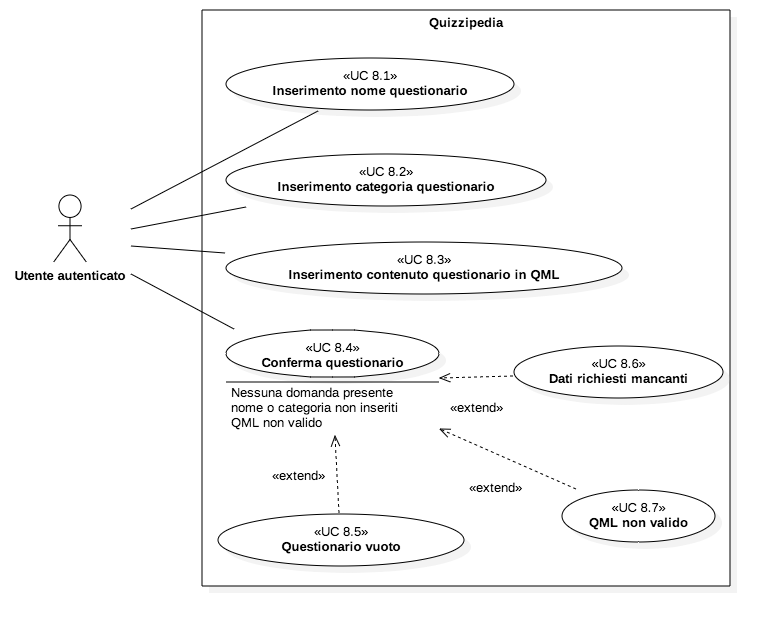
\includegraphics[scale=0.45]{../immagini/UC8.png}
\caption{Creazione questionario}
\end{figure}
\ \\
\textbf{Attori:} \textit{utente autenticato}
\\ \\
\textbf{Descrizione:} caso d'uso che descrive la creazione di un nuovo questionario.\\
\\
\textbf{Precondizioni:} l'utente può creare un questionario.\\
\\
\textbf{Postcondizioni:} l’utente ha creato un nuovo questionario.\\
\\
\textbf{Scenario:} l’utente inserisce i dati del questionario (UC 8.1, UC 8.2, UC 8.4, UC 8.8) e li invia al sistema che memorizza il nuovo questionario (UC 8.5). L'inserimento della categoria fa visualizzare la lista delle domande relative a quella categoria (UC 8.3). Se all'invio il questionario risulta vuoto o alcuni dati essenziali mancano viene visualizzato un messaggio di errore (UC 8.6, UC 8.7). In ogni momento l'utente può uscire e annullare l'operazione.\\


\subsubsection{UC 8.1 - Inserimento nome questionario}

\textbf{Attori:} \textit{utente autenticato}
\\ \\
\textbf{Descrizione:} caso d'uso che descrive l'inserimento del nome del questionario.\\
\\
\textbf{Precondizioni:} il sistema permette l'inserimento di un nome.\\
\\
\textbf{Postcondizioni:} l’utente ha inserito il nome del questionario.\\
\\
\textbf{Scenario:} l’utente inserisce il nome del questionario nell'apposito campo.\\


\subsubsection{UC 8.2 - Inserimento categoria questionario}

\textbf{Attori:} \textit{utente autenticato}
\\ \\
\textbf{Descrizione:} caso d'uso che descrive l'inserimento della categoria del questionario.\\
\\
\textbf{Precondizioni:} il sistema permette l'inserimento di una categoria.\\
\\
\textbf{Postcondizioni:} l’utente ha inserito la categoria del questionario. Vengono visualizzate le domande relative a quella categoria.\\
\\
\textbf{Scenario:} l’utente inserisce la categoria del questionario nell'apposito campo.\\


\subsubsection{UC 8.3 - Visualizzazione lista domande}

\textbf{Attori:} \textit{utente autenticato}
\\ \\
\textbf{Descrizione:} caso d'uso che descrive la visualizzazione della lista delle domande.\\
\\
\textbf{Precondizioni:} l'utente ha selezionato una categoria.\\
\\
\textbf{Postcondizioni:} l’utente visualizza le domande relative a quella categoria e può selezionarle.\\
\\
\textbf{Scenario:} l’utente ha inserito la categoria del questionario nell'apposito campo. Il sistema visualizza i testi delle domande della categoria inserita.\\


\subsubsection{UC 8.4 - Selezione domanda}

\textbf{Attori:} \textit{utente autenticato}
\\ \\
\textbf{Descrizione:} caso d'uso che descrive la selezione di una domanda dalla lista.\\
\\
\textbf{Precondizioni:} l'utente ha selezionato una categoria e visualizza una lista di domande.\\
\\
\textbf{Postcondizioni:} l’utente ha selezionato una domanda dalla lista.\\
\\
\textbf{Scenario:} l'utente seleziona una domanda dalla lista.\\


\subsubsection{UC 8.5 - Conferma questionario}

\textbf{Attori:} \textit{utente autenticato}
\\ \\
\textbf{Descrizione:} caso d'uso che descrive l'invio dei dati del nuovo questionario.\\
\\
\textbf{Precondizioni:} l'utente ha inserito i dati del questionario.\\
\\
\textbf{Postcondizioni:} l’utente ha inviato i dati del questionario e il sistema l'ha memorizzato nel database.\\
\\
\textbf{Scenario:} l’utente invia i dati del questionario. Il sistema memorizza nel database il nuovo questionario.\\
\\
\textbf{Extension points:} 
\begin{itemize}
	\item \textbf{Questionario vuoto:} l'utente non ha inserito nessuna domanda nel questionario, viene visualizzato un messaggio di errore (UC 8.6)
	\item \textbf{Dati richiesti mancanti:} il nome e/o la categoria del questionario non sono stati inseriti dall'utente, viene visualizzato un messaggio di errore (UC 8.7)
\end{itemize}


\subsubsection{UC 8.6 - Questionario vuoto}

\textbf{Attori:} \textit{utente autenticato}
\\ \\
\textbf{Descrizione:} caso d'uso che descrive la visualizzazione del messaggio di errore relativo alla creazione di un questionario vuoto.\\
\\
\textbf{Precondizioni:} l'utente ha confermato la creazione del questionario. Nessuna domanda è presente nel questonario.\\
\\
\textbf{Postcondizioni:} l’utente visualizza il messaggio di errore relativo alla creazione di un questionario vuoto.\\
\\
\textbf{Scenario:} l'utente conferma la creazione di un questionario vuoto e visualizza il messaggio di errore relativo alla creazione di un questionario vuoto.\\


\subsubsection{UC 8.7 - Dati richiesti questionario mancanti}

\textbf{Attori:} \textit{utente autenticato}
\\ \\
\textbf{Descrizione:} caso d'uso che descrive la visualizzazione del messaggio di errore relativo alla mancanza di dati necessari.\\
\\
\textbf{Precondizioni:} l'utente ha confermato la creazione del questionario. Almeno un dato necessario alla creazione non è stato inserito.\\
\\
\textbf{Postcondizioni:} l’utente visualizza il messaggio di errore relativo alla mancanza di dati necessari.\\
\\
\textbf{Scenario:} l'utente conferma la creazione di un questionario senza inserire almeno una informazione necessaria e visualizza il relativo messaggio di errore.\\


\subsubsection{UC 8.8 - Inserimento tempo di compilazione}

\textbf{Attori:} \textit{utente autenticato}
\\ \\
\textbf{Descrizione:} caso d'uso che descrive l'inserimento del tempo di compilazione del questionario.\\
\\
\textbf{Precondizioni:} il sistema permette l'inserimento di un tempo di compilazione.\\
\\
\textbf{Postcondizioni:} l’utente ha inserito il tempo di compilazione del questionario.\\
\\
\textbf{Scenario:} l'utente inserisce il tempo di compilazione del questionario nell'apposito campo.\\


\subsection{UC 9 - Logout}

\textbf{Attori:} \textit{utente autenticato}
\\ \\
\textbf{Descrizione:} caso d'uso che descrive il logout dell'utente.\\
\\
\textbf{Precondizioni:} il sistema permette il logout.\\
\\
\textbf{Postcondizioni:} l’utente non è più autenticato.\\
\\
\textbf{Scenario:} l’utente clicca su logout. Il sistema non riconosce più come autenticato l'utente.\\


\newpage
\subsection{UC 10 - Ricerca questionario}

\begin{figure}[h!]
\centering
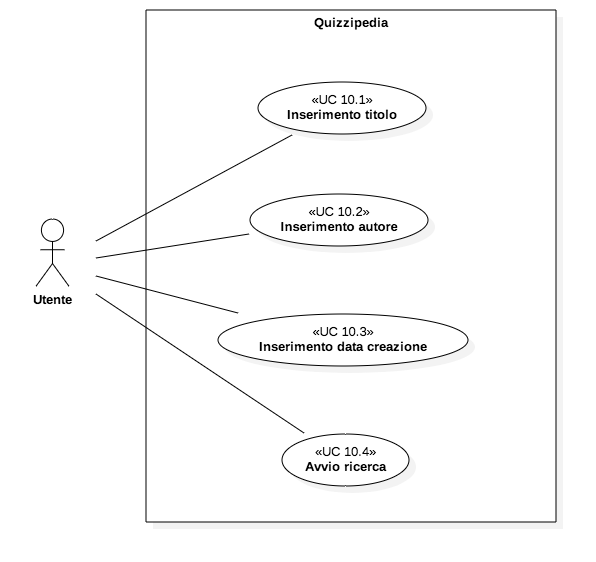
\includegraphics[scale=0.60]{../immagini/UC10.png}
\caption{Ricerca questionario}
\end{figure}
\ \\
\textbf{Attori:} \textit{utente}
\\ \\
\textbf{Descrizione:} caso d'uso che descrive la ricerca di questionari.\\
\\
\textbf{Precondizioni:} l'utente può fare una ricerca di questionari.\\
\\
\textbf{Postcondizioni:} l’utente visualizza una lista di questionari.\\
\\
\textbf{Scenario:} l’utente inserisce i dati dei questionari da ricercare (UC 10.1, UC 10.2, UC 10.3), poi avvia la ricerca (UC 10.4) e visualizza i risultati (UC 4).\\


\subsubsubsection{UC 10.1 - Inserimento titolo}

\textbf{Attori:} \textit{utente}
\\ \\
\textbf{Descrizione:} caso d'uso che descrive l'inserimento del titolo dei questionari da cercare.\\
\\
\textbf{Precondizioni:} l'utente sta effettuando una ricerca di questionari.\\
\\
\textbf{Postcondizioni:} l’utente ha inserito il titolo dei questionari da cercare.\\
\\
\textbf{Scenario:} l’utente inserisce il titolo nell'apposito campo per la ricerca.\\


\subsubsubsection{UC 10.2 - Inserimento autore}

\textbf{Attori:} \textit{utente}
\\ \\
\textbf{Descrizione:} caso d'uso che descrive l'inserimento dell'autore dei questionari da cercare.\\
\\
\textbf{Precondizioni:} l'utente sta effettuando una ricerca di questionari.\\
\\
\textbf{Postcondizioni:} l’utente ha inserito l'autore dei questionari da cercare.\\
\\
\textbf{Scenario:} l’utente inserisce l'autore nell'apposito campo per la ricerca.\\


\subsubsubsection{UC 10.3 - Inserimento data di creazione}

\textbf{Attori:} \textit{utente}
\\ \\
\textbf{Descrizione:} caso d'uso che descrive l'inserimento dalla data di creazione dei questionari da cercare.\\
\\
\textbf{Precondizioni:} l'utente sta effettuando una ricerca di questionari.\\
\\
\textbf{Postcondizioni:} l’utente ha inserito la data di creazione dei questionari da cercare.\\
\\
\textbf{Scenario:} l’utente inserisce la data di creazione nell'apposito campo per la ricerca.\\


\subsubsubsection{UC 10.4 - Avvio ricerca}

\textbf{Attori:} \textit{utente}
\\ \\
\textbf{Descrizione:} caso d'uso che descrive la ricerca di questionari.\\
\\
\textbf{Precondizioni:} l'utente vuole effettuare una ricerca di questionari.\\
\\
\textbf{Postcondizioni:} l’utente visualizza la lista di questionari che rispettano i criteri inseriti.\\
\\
\textbf{Scenario:} l’utente avvia la ricerca e visualizza la lista di questionari che soddisfano i criteri inseriti.\\	
	\newpage

\subsection{UC 11 - Recupero password}

\begin{figure}[h!]
\centering
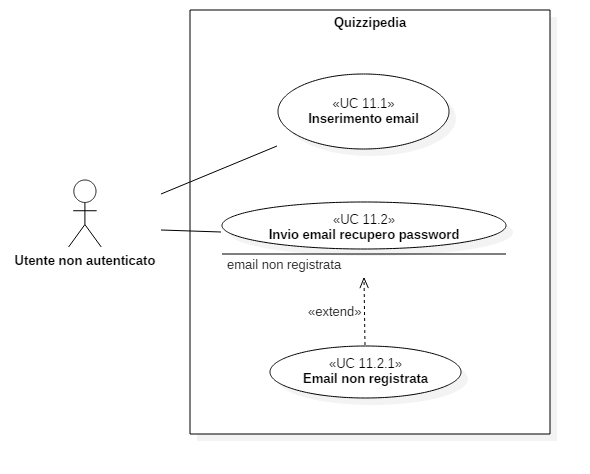
\includegraphics[scale=0.6]{../immagini/UC11.png}
\caption{Procedura per il recupero della password}
\end{figure}
\ \\
\textbf{Attori:} \textit{utente non autenticato}
\\ \\
\textbf{Descrizione:} caso d'uso che descrive la procedura di recupero password in caso di dimenticanza.\\
\\
\textbf{Precondizioni:} l'utente non ricorda più la propria password.\\
\\
\textbf{Postcondizioni:} l’utente ha recuperato la propria password.\\
\\
\textbf{Scenario:} l’utente segue la procedura di recupero password e il sistema provvede a mandare una email con la password all'utente.\\


\subsubsubsection{UC 11.1 - Inserimento email}

\textbf{Attori:} \textit{utente non autenticato}
\\ \\
\textbf{Descrizione:} caso d'uso che descrive l'inserimento della email nella procedura di recupero password.\\
\\
\textbf{Precondizioni:} l'utente è nella procedura di recupero password.\\
\\
\textbf{Postcondizioni:} l’utente ha inserito la propria email.\\
\\
\textbf{Scenario:} l’utente inserisce la propria email nell'apposito campo.\\


\subsubsubsection{UC 11.2 - Invio email recupero password}

\textbf{Attori:} \textit{utente non autenticato}
\\ \\
\textbf{Descrizione:} caso d'uso che descrive l'invio al sistema della email nella procedura di recupero password.\\
\\
\textbf{Precondizioni:} l'utente ha inserito la propria email nella procedura di recupero password.\\
\\
\textbf{Postcondizioni:} l’utente riceve una email con la propria password dimenticata.\\
\\
\textbf{Scenario:} l’utente invia la propria email e il sistema manda una mail con la password dimenticata.\\
\\
\textbf{Extension points:} 
\begin{itemize}
	\item \textbf{Email non registrata:} La email inviata al sistema non corrisponde a nessun utente, viene visualizzato un messaggio di errore (UC 11.2.1)
\end{itemize}
	\newpage

\section{Requisiti}
		Di seguito vengono elencati i requisiti emersi in fase di analisi del capitolato e del problema.\\
		I requisiti sono presentati in maniera gerarchica affinché i sotto-requisiti specifichino ulteriori informazioni e dettagli rispetto al loro genitore.\\
		Per avere una migliore organizzazione dei requisiti questi vengono suddivisi in funzionali (F), QML (QML), di qualità (Q) e vincoli di sistema imposti dal capitolato (V).\\
		Dopo la categoria ogni codice identificativo è completato da un numero che mostra anche il livello e l'appartenenza della gerarchia sopra descritta.\\
		\subsection{Requisiti funzionali}
			\begin{longtable}{p{0.2\columnwidth}p{0.6\textwidth}p{0.2\columnwidth}}
			\caption{Requisiti funzionali} \\

ID & Descrizione & Priorità \\
\midrule
\endfirsthead

ID & Descrizione & Priorità \\
\midrule
\endhead

\multicolumn{2}{c}{\footnotesize\itshape\tablename~\thetable: Requisiti funzionali}
\endfoot

\multicolumn{2}{c}{\footnotesize\itshape\tablename~\thetable: Requisiti funzionali}
\endlastfoot

F 1 & Il sistema deve fornire la possibilità ad un utente non autenticato di registrarsi & Obbligatorio\\
\midrule
F 1.1 & La sezione dedicata alla registrazione deve permettere l'inserimento dei dati necessari & Obbligatorio\\
\midrule
F 1.1.1 & La sezione dedicata alla registrazione deve permettere l'inserimento di una email & Obbligatorio\\
\midrule
F 1.1.2 & La sezione dedicata alla registrazione deve permettere l'inserimento di una password & Obbligatorio\\
\midrule
F 1.1.2.1 & Se la password inserita ha meno di 8 caratteri viene visualizzato un messaggio di errore & Desiderabile\\
\midrule
F 1.2 & La sezione dedicata alla registrazione deve permettere l'invio dei dati inseriti & Obbligatorio\\
\midrule
F 1.2.1 & Prima di inviare i dati viene effettuato un controllo su di essi & Obbligatorio\\
\midrule
F 1.2.1.1 & Se i dati richiesti non sono stati inseriti viene visualizzato un messaggio di errore & Desiderabile\\
\midrule
F 1.2.1.2 & Se la email inserita risulta già in uso viene visualizzato un messaggio di errore & Desiderabile\\
\midrule
F 1.2.1.3 & Se i dati non risultano corretti ne viene bloccato l'invio & Obbligatorio\\
\midrule
F 1.2.2 & Quando dei dati corretti vengono inviati il sistema memorizza un nuovo account con essi & Obbligatorio\\
\midrule
F 1.2.3 & Quando viene creato un nuovo account con la procedura di registrazione viene automaticamente effettuato il login con quell'account & Desiderabile\\
\midrule
F 2 & Il sistema deve fornire la possibilità ad un utente non autenticato di autenticarsi & Obbligatorio\\
\midrule
F 2.1 & La sezione dedicata all'autenticazione deve permettere l'inserimento dei dati necessari & Obbligatorio\\
\midrule
F 2.1.1 & La sezione dedicata all'autenticazione deve permettere l'inserimento di una email & Obbligatorio\\
\midrule
F 2.1.2 & La sezione dedicata all'autenticazione deve permettere l'inserimento di una password & Obbligatorio\\
\midrule
F 2.2 & La sezione dedicata all'autenticazione deve fornire una procedura di recupero password & Facoltativo\\
\midrule
F 2.2.1 & La procedura di recupero password deve permettere l'inserimento della email & Facoltativo\\
\midrule
F 2.2.2 & La procedura di recupero password deve effettuare un controllo sulla email inserita & Facoltativo\\
\midrule
F 2.2.2.1 & Se la email non risulta registrata viene visualizzato un messaggio di errore & Facoltativo\\
\midrule
F 2.2.2.2 & Se la email non risulta registrata viene bloccato l'invio della mail a quell'indirizzo & Facoltativo\\
\midrule
F 2.2.3 & La procedura di recupero password deve mandare una mail all'indirizzo inserito con la password dimenticata & Facoltativo\\
\midrule
F 2.3 & La sezione dedicata all'autenticazione deve permettere l'invio dei dati inseriti & Obbligatorio\\
\midrule
F 2.3.1 & Prima di inviare i dati viene effettuato un controllo su di essi & Obbligatorio\\
\midrule
F 2.3.1.1 & Se la combinazione email/password non è registrata viene visualizzato un messaggio di errore & Desiderabile\\
\midrule
F 2.3.2 & Se la combinazione email/password è registrata l'utente viene autenticato & Obbligatorio\\
\midrule
F 3 & Il sistema deve permettere la navigazione dei questionari per categoria & Obbligatorio\\
\midrule
F 3.1 & Il sistema deve fornire una sezione con un elenco delle categorie di questionari presenti nel database & Obbligatorio\\
\midrule
F 3.1.1 & Quando l'utente seleziona una categoria viene visualizzata la sezione che elenca i questionari della categoria scelta & Obbligatorio\\
\midrule
F 3.1.2 & Per ogni elemento dell'elenco viene visualizzato il nome della categoria & Obbligatorio\\
\midrule
F 3.1.3 & Per ogni elemento dell'elenco viene visualizzato il numero di questionari della categoria & Facoltativo\\
\midrule
F 3.2 & Il sistema deve fornire una sezione con un elenco dei questionari relativi ad una categoria & Obbligatorio\\
\midrule
F 3.2.1 & Quando l'utente seleziona un questionario viene visualizzata la sezione della compilazione del questionario scelto & Obbligatorio\\
\midrule
F 3.2.2 & Per ogni elemento dell'elenco viene visualizzato il nome del questionario & Obbligatorio\\
\midrule
F 3.2.3 & Per ogni elemento dell'elenco viene visualizzato il numero di domande del questionario & Facoltativo\\
\midrule
F 3.2.4 & Per ogni elemento dell'elenco viene visualizzato l'autore & Facoltativo\\
\midrule
F 3.2.5 & Per ogni elemento dell'elenco viene visualizzato la data di creazione & Facoltativo\\
\midrule
F 3.3 & Il sistema deve permettere all'utente la ricerca di un determinato questionario & Desiderabile\\
\midrule
F 3.3.1 & Il sistema deve permettere all'utente la ricerca per nome & Desiderabile\\
\midrule
F 3.3.2 & Il sistema deve permettere all'utente la ricerca per numero di domande & Desiderabile\\
\midrule
F 3.3.3 & Il sistema deve permettere all'utente la ricerca per popolarità & Facoltativo\\
\midrule
F 4 & Il sistema deve fornire la possibilità di compilare un questionario & Obbligatorio\\
\midrule
F 4.1 & Durante la compilazione del questionario un utente può navigare liberamente tra le domande che lo compongono & Desiderabile\\
\midrule
F 4.1.1 & Durante lo svolgimento di un questionario viene presentato un singolo quesito per volta all'utente & Desiderabile\\
\midrule
F 4.2 & L'utente può rispondere alle domande & Obbligatorio\\
\midrule
F 4.2.1 & Viene visualizzato il testo della domanda & Obbligatorio\\
\midrule
F 4.2.2 & Viene visualizzata la risposta data & Obbligatorio\\
\midrule
F 4.2.3 & Se la domanda richiede una risposta inserita dall'utente allora viene fornito un campo per l'inserimento della risposta & Obbligatorio\\
\midrule
F 4.2.4 & Se la domanda ha delle risposte preimpostate di qualsiasi tipo queste vengono visualizzate & Obbligatorio\\
\midrule
F 4.2.4.1 & Deve essere possibile selezionare una risposta & Obbligatorio\\
\midrule
F 4.2.5 & Se la domanda permette associazioni tra elementi deve visualizzare tutti gli elementi associabili & Facoltativo\\
\midrule
F 4.2.5.1 & Deve essere possibile associare due elementi di insiemi diversi & Facoltativo\\
\midrule
F 4.2.6 & Se la domanda prevede il completamento del testo con delle parole vengono visualizzate le possibili parole & Facoltativo\\
\midrule
F 4.2.6.1 & Deve essere possibile selezionare una parola dalla lista & Facoltativo\\
\midrule
F 4.3 & L'utente può cambiare la risposta di una domanda in qualsiasi momento prima della consegna del questionario & Desiderabile\\
\midrule
F 4.4 & Le domande possono essere compilate in un ordine qualsiasi & Desiderabile\\
\midrule
F 4.5 & L'utente può consegnare il questionario & Obbligatorio\\
\midrule
F 4.5.1 & Se alla consegna una o più domande non sono state compilate il sistema avverte l'utente di ciò & Desiderabile\\
\midrule
F 4.5.2 & Quando un questionario viene confermato e consegnato viene valutato dal sistema & Obbligatorio\\
\midrule
F 4.5.2.1 & La valutazione del questionario viene visualizzata all'utente & Obbligatorio\\
\midrule
F 4.5.2.1.1 & Viene visualizzato il nome del questionario & Obbligatorio\\
\midrule
F 4.5.2.1.2 & Viene visualizzato il punteggio ottenuto & Obbligatorio\\
\midrule
F 4.5.2.1.3 & Viene visualizzata la percentuale delle risposte corrette & Desiderabile\\
\midrule
F 4.6 & La compilazione del questionario ha un tempo massimo & Facoltativo\\
\midrule
F 4.6.1 & Allo scadere del tempo il questionario verrà consegnato automaticamente anche se incompleto & Facoltativo\\
\midrule
F 4.6.2 & Il tempo inizia a scorrere da quando l'utente accede alla pagina & Facoltativo\\
\midrule
F 4.7 & Viene visualizzato il tempo restante & Facoltativo\\
\midrule
F 5 & Il sistema deve fornire la possibilità ad un utente autenticato di creare una nuova domanda & Obbligatorio\\
\midrule
F 5.1 & La sezione dedicata alla creazione di una domanda deve permettere l'inserimento dei dati necessari & Obbligatorio\\
\midrule
F 5.1.1 & La sezione dedicata alla creazione di una domanda deve permettere la scelta di una o più categorie & Obbligatorio\\
\midrule
F 5.1.2 & La sezione dedicata alla creazione di una domanda deve permettere l'inserimento del codice QML che definisce la domanda & Obbligatorio\\
\midrule
F 5.2 & La sezione dedicata alla creazione di una domanda deve permettere l'invio dei dati inseriti & Obbligatorio\\
\midrule
F 5.2.1 & Prima di inviare i dati viene effettuato un controllo su di essi & Obbligatorio\\
\midrule
F 5.2.1.1 & Se i dati obbligatori non risultano inseriti viene visualizzato un messaggio di errore & Desiderabile\\
\midrule
F 5.2.1.2 & Se il codice QML inserito non risulta valido viene visualizzato un messaggio di errore & Desiderabile\\
\midrule
F 5.2.1.3 & Se i dati obbligatori non risultano inseriti o il codice QML non è valido la creazione della nuova domanda viene bloccata & Obbligatorio\\
\midrule
F 5.2.2 & Quando dei dati che superano i controlli vengono inviati viene creata una nuova domanda con essi e inserita nel database & Obbligatorio\\
\midrule
F 5.2.2.1 & Se la creazione di una nuova domanda va a buon fine il sistema avvisa l'utente & Desiderabile\\
\midrule
F 5.2.2.2 & Se la creazione di una nuova domanda non va a buon fine il sistema visualizza un messaggio di errore & Desiderabile\\
\midrule
F 5.3 & L'utente ha la possibilità di modificare domande da lui precedentemente create & Facoltativo\\
\midrule
F 5.3.1 & Qualora la modifica venga ritenuta valida essa viene salvata e l'utente ne viene notificato & Facoltativo\\
\midrule
F 5.3.2 & Qualora la modifica non venga ritenuta conforme l'utente viene avvertito da un messaggio d'errore & Facoltativo\\
\midrule
F 5.4 & L'utente ha la possibilità di eliminare domande da lui precedentemente create & Facoltativo\\
\midrule
F 5.5 & L'utente ha la possibilità di annullare alcune operazioni effettuate & Facoltativo\\
\midrule
F 5.5.1 & L'utente ha la possibilità di annullare la creazione di una domanda & Facoltativo\\
\midrule
F 5.5.2 & L'utente ha la possibilità di annullare la modifica di una domanda & Facoltativo\\
\midrule
F 5.5.3 & L'utente ha la possibilità di annullare l'eliminazione di una domanda & Facoltativo\\
\midrule
F 6 & Il sistema deve fornire la possibilità ad un utente autenticato di creare un nuovo questionario & Obbligatorio\\
\midrule
F 6.1 & La sezione dedicata alla creazione di un questionario deve permettere l'inserimento dei dati necessari & Obbligatorio\\
\midrule
F 6.1.1 & La sezione dedicata alla creazione di un questionario deve permettere l'inserimento del nome del questionario & Obbligatorio\\
\midrule
F 6.1.2 & La sezione dedicata alla creazione di un questionario deve permettere l'inserimento della categoria del questionario & Obbligatorio\\
\midrule
F 6.1.3 & La sezione dedicata alla creazione di un questionario deve visualizzare la lista delle domande della categoria selezionata & Obbligatorio\\
\midrule
F 6.1.3.1 & Se nessuna categoria è stata selezionata non viene visualizzata alcuna domanda & Obbligatorio\\
\midrule
F 6.1.3.2 & Ogni domanda deve essere selezionabile & Obbligatorio\\
\midrule
F 6.1.4 & La sezione dedicata alla creazione di un questionario deve permettere il regolamento del tempo limite per la compilazione & Facoltativo\\
\midrule
F 6.1.4.1 & Il tempo limite minimo per la compilazione del questionario è di 5 (cinque) minuti & Facoltativo\\
\midrule
F 6.1.4.2 & Il tempo limite massimo per la compilazione del questionario è di 30 (trenta) minuti & Facoltativo\\
\midrule
F 6.1.4.3 & Qualora l'utente non lo specificasse, il tempo limite di default per la compilazione del questionario è di 10 (dieci) minuti & Facoltativo\\
\midrule
F 6.2 & La sezione dedicata alla creazione di un nuovo questionario deve permettere l'invio dei dati inseriti & Obbligatorio\\
\midrule
F 6.2.1 & Prima di inviare i dati viene effettuato un controllo su di essi & Obbligatorio\\
\midrule
F 6.2.1.1 & Se i dati obbligatori non risultano inseriti viene visualizzato un messaggio di errore & Desiderabile\\
\midrule
F 6.2.1.2 & Se nessuna domanda è selezionata viene visualizzato un messaggio di errore & Desiderabile\\
\midrule
F 6.2.1.3 & Se i dati obbligatori non risultano inseriti non è valido nessun dato viene inviato & Obbligatorio\\
\midrule
F 6.2.2 & Quando dei dati che superano i controlli vengono inviati viene creato un nuovo questionario con essi e inserito nel database & Obbligatorio\\
\midrule
F 6.2.2.1 & Se la creazione di un nuovo questionario va a buon fine il sistema avvisa l'utente & Desiderabile\\
\midrule
F 6.2.2.2 & Se la creazione di un nuovo questionario non va a buon fine il sistema visualizza un messaggio di errore & Desiderabile\\
\midrule
F 6.2.3 & La sezione dedicata alla creazione di un nuovo questionario deve permetterne l'annullamento qualora l'utente abbia ripensamenti & Facoltativo\\
\midrule
F 7 & Il sistema deve fornire la possibilità ad un utente autenticato di uscire facendo il logout & Obbligatorio\\
\midrule
F 8 & Il sistema deve essere in grado di interpretare il codice QML & Obbligatorio\\
\midrule
F 8.1 & QML definisce domande & Obbligatorio\\
\midrule
F 8.1.1 & Una domanda è formata dal testo del quesito e da una o più risposte & Obbligatorio\\
\midrule
F 8.1.2 & Una domanda deve avere almeno una risposta esatta & Obbligatorio\\
\midrule
F 8.1.3 & Una domanda può avere una lista di possibili risposte & Obbligatorio\\
\midrule
F 8.1.4 & QML permette la definizione di diverse tipologie di domande & Obbligatorio\\
\midrule
F 8.1.4.1 & QML definisce domande di tipo vero o falso & Obbligatorio\\
\midrule
F 8.1.4.2 & QML definisce domande a scelta multipla con una sola risposta esatta & Obbligatorio\\
\midrule
F 8.1.4.3 & QML definisce domande a scelta multipla con più risposte esatte & Desiderabile\\
\midrule
F 8.1.4.4 & QML definisce domande a risposta testuale & Obbligatorio\\
\midrule
F 8.1.4.5 & QML definisce domande di associazione tra elementi di due insiemi & Desiderabile\\
\midrule
F 8.1.4.5.1 & Gli insiemi possono contenere elementi non associabili di disturbo & Facoltativo\\
\midrule
F 8.1.4.6 & QML definisce domande a completamento testuale a scelta da un gruppo di parole date & Facoltativo\\
\midrule
F 8.1.4.6.1 & Il gruppo di parole può contenere elementi di disturbo & Facoltativo\\
\midrule
F 8.1.4.7 & QML definisce domande di associazione tra date poste in una timeline e avvenimenti & Facoltativo\\
\midrule
F 8.2 & QML gestisce immagini all'interno di domande e risposte preimpostate & Desiderabile\\
\midrule
F 8.3 & All'interno della piattaforma Quizzipedia è presente un regolamento sull'utilizzo della sintassi QML & Desiderabile\\			
			\end{longtable}
		\subsection{Requisiti di qualità}
			\begin{longtable}{p{0.2\columnwidth}p{0.6\textwidth}p{0.2\columnwidth}}
			\caption{Requisiti di qualità} \\

ID & Descrizione & Priorità \\
\midrule
\endfirsthead

ID & Descrizione & Priorità \\
\midrule
\endhead

\multicolumn{2}{c}{\footnotesize\itshape\tablename~\thetable: Requisiti di qualità}
\endfoot

\multicolumn{2}{c}{\footnotesize\itshape\tablename~\thetable: Requisiti di qualità}
\endlastfoot
			
Q 1 & Ogni file contiene codice scritto in un solo linguaggio per separare struttura, contenuto e comportamento & Obbligatorio\\
\midrule
Q 1.1 & Il codice HTML si occupa della struttura delle pagine web & Obbligatorio\\
\midrule
Q 1.2 & Il codice CSS si occupa dello stile delle pagine web & Obbligatorio\\
\midrule
Q 1.3 & Il codice Javascript si occupa del comportamento delle pagine web & Obbligatorio\\
\midrule
Q 2 & Il codice HTML passa il test di validazione del W3C & Obbligatorio\\
\midrule
Q 3 & Il codice CSS passa il test di validazione del W3C & Obbligatorio\\
\midrule
Q 4 & E' presente un manuale sul futuro mantenimento del sistema per uno sviluppatore esterno & Desiderabile\\
\midrule
Q 5 & E' presente un manuale sull'utilizzo del sistema per l'utente & Desiderabile\\
			
			\end{longtable}
		\subsection{Vincoli di sistema}
			\begin{longtable}{p{0.2\columnwidth}p{0.6\textwidth}p{0.2\columnwidth}}
			\caption{Vincoli di sistema} \\

ID & Descrizione & Priorità \\
\midrule
\endfirsthead

ID & Descrizione & Priorità \\
\midrule
\endhead

\multicolumn{2}{c}{\footnotesize\itshape\tablename~\thetable: Vincoli di sistema}
\endfoot

\multicolumn{2}{c}{\footnotesize\itshape\tablename~\thetable: Vincoli di sistema}
\endlastfoot
			
V 1 & Il sistema deve essere utilizzabile attraverso un browser che supporti HTML 5, CSS 3 e Javascript & Obbligatorio\\
\midrule
V 1.1 & L'interfaccia utente deve essere fruibile via desktop, tablet e smartphone & Obbligatorio\\
\midrule
V 1.2 & L'interfaccia utente deve essere strutturata con HTML 5 & Obbligatorio\\
\midrule
V 1.3 & Lo stile dell'interfaccia utente deve essere realizzato tramite fogli di stile CSS 3 & Obbligatorio\\
\midrule
V 1.4 & La parte attiva dell'interfaccia utente deve essere gestita utilizzando Javascript & Obbligatorio\\
\midrule
V 2 & Domande vengono gestiti con il linguaggio QML & Obbligatorio\\
\midrule
V 3 & La parte server viene realizzata in Javascript con server Node.js & Obbligatorio\\
\midrule
V 3.1 & La base di dati sarà non relazione e verrà implementata utilizzando MongoDB & Desiderabile\\
\midrule
V 3.2 & I dati verranno memorizzati in formato JSON & Desiderabile\\
\midrule
V 4 & L' intero sistema verrà dimensionato attenendosi alle linee guida imposte dai framework Meteor e AngularJS & Desiderabile\\
\midrule
V 4.1 & Il sistema Quizzipedia dovrà essere compatibile con i seguenti browser: Android stock browser (Webkit based), Chrome, Firefox 7+, iOS browser, IE8+, Safari 4+, Desktop Opera, Mobile Opera & Desiderabile\\
			
			\end{longtable}
	
	\newpage
	\section{Mappature}
		\subsection{Mappatura casi d'uso - requisiti}
			\begin{longtable}{p{0.5\columnwidth}p{0.5\textwidth}}
			\caption{Mappatura casi d'uso - requisiti} \\

Caso d'uso & Requisito \\
\midrule
\endfirsthead

Caso d'uso & Requisito \\
\midrule
\endhead

\multicolumn{2}{c}{\footnotesize\itshape\tablename~\thetable: Mappatura casi d'uso - requisiti}
\endfoot

\multicolumn{2}{c}{\footnotesize\itshape\tablename~\thetable: Mappatura casi d'uso - requisiti}
\endlastfoot
			
UC 1 & F 2\\
\midrule
UC 1.1 & F 2.1, F 2.1.1\\
\midrule
UC 1.2 & F 2.1, F 2.1.2\\
\midrule
UC 1.3 & F 2.2\\
\midrule
UC 1.3.1 & F 2.2.1\\
\midrule
UC 1.3.2 & F 2.2.2, F 2.2.3\\
\midrule
UC 1.3.3 & F 2.2.2.1, F 2.2.2.2\\
\midrule
UC 1.4 & F 2.3, F 2.3.1, F 2.3.2\\
\midrule
UC 1.5 & F 2.3.1.1\\
\midrule
UC 2 & F 1\\
\midrule
UC 2.1 & F 1.1, F 1.1.1\\
\midrule
UC 2.2 & F 1.1, F 1.1.2\\
\midrule
UC 2.3 & F 1.1.2.1\\
\midrule
UC 2.4 & F 1.2, F 1.2.1, F 1.2.2, F 1.2.3\\
\midrule
UC 2.5 & F 1.2.1.1, F 1.2.1.3\\
\midrule
UC 2.6 & F 1.2.1.2, F 1.2.1.3\\
\midrule
UC 3 & F 3, F 3.1\\
\midrule
UC 3.1 & F 3.1.2\\
\midrule
UC 3.2 & F 3.1.3\\
\midrule
UC 4 & F 3.1.1, F 3.2, F 3.2.1\\
\midrule
UC 4.1 & F 3.2.2\\
\midrule
UC 4.2 & F 3.2.3\\
\midrule
UC 4.3 & F 3.2.4\\
\midrule
UC 5 & F 3.2.1\\
\midrule
UC 6 & F 4\\
\midrule
UC 6.1 & F 4.2.1, F 4.2.1, F 4.2.2, F 4.2.4, F 4.2.5, F 4.2.6\\
\midrule
UC 6.1.1 & F 4.2.1\\
\midrule
UC 6.1.2 & F 4.2.4, F 4.2.5, F 4.2.6\\
\midrule
UC 6.1.3 & F 4.2.2\\
\midrule
UC 6.2 & F 4.2, F 4.3\\
\midrule
UC 6.2.1 & F 4.2.4.1\\
\midrule
UC 6.2.2 & F 4.2.3\\
\midrule
UC 6.2.3 & F 4.2.5.1\\
\midrule
UC 6.2.4 & F 4.2.6.1\\
\midrule
UC 6.2.5 & F 4.2.5.1\\
\midrule
UC 6.3 & F 4.5\\
\midrule
UC 6.4 & F 4.5.1\\
\midrule
UC 6.5 & F 4.5.2\\
\midrule
UC 6.5.1 & F 4.5.2.1.1\\
\midrule
UC 6.5.2 & F 4.5.2.1.2\\
\midrule
UC 6.5.3 & F 4.5.2.1.3\\
\midrule
UC 6.6 & F 4.6, F 4.7\\
\midrule
UC 7 & F 5\\
\midrule
UC 7.1 & F 5.1, F 5.1.1\\
\midrule
UC 7.2 & F 5.1, F 5.1.2\\
\midrule
UC 7.3 & F 5.2, F 5.2.1, F 5.2.2, F 5.2.2.1, F 5.2.2.2\\
\midrule
UC 7.4 & F 5.2.1.1, F 5.2.1.3\\
\midrule
UC 7.5 & F 5.2.1.2, F 5.2.1.3\\
\midrule
UC 8 & F 6\\
\midrule
UC 8.1 & F 6.1, F 6.1.1\\
\midrule
UC 8.2 & F 6.1, F 6.1.2\\
\midrule
UC 8.3 & F 6.1, F 6.1.3, F 6.1.3.1\\
\midrule
UC 8.4 & F 6.1, F 6.1.3.1\\
\midrule
UC 8.5 & F 6.2, F 6.2.1, F 6.2.2, F 6.2.2.1, F 6.2.2.2\\
\midrule
UC 8.6 & F 6.2.1.2, F 6.2.1.3\\
\midrule
UC 8.7 & F 6.2.1.1, F 6.2.1.3\\
\midrule
UC 9 & F 7\\
		
			
			\end{longtable}

		\subsection{Mappatura requisiti - casi d'uso}
			\begin{longtable}{p{0.5\columnwidth}p{0.5\textwidth}}
			\caption{Mappatura requisiti - casi d'uso} \\

Requisito & Caso d'uso \\
\midrule
\endfirsthead

Requisito & Caso d'uso \\
\midrule
\endhead

\multicolumn{2}{c}{\footnotesize\itshape\tablename~\thetable: Mappatura requisiti - casi d'uso}
\endfoot

\multicolumn{2}{c}{\footnotesize\itshape\tablename~\thetable: Mappatura requisiti - casi d'uso}
\endlastfoot
			
F 1 & UC 2\\
\midrule
F 1.1 & UC 2.1, UC 2.2\\
\midrule
F 1.1.1 & UC 2.1\\
\midrule
F 1.1.2 & UC 2.2\\
\midrule
F 1.1.2.1 & UC 2.3\\
\midrule
F 1.2 & UC 2.4\\
\midrule
F 1.2.1 & UC 2.4\\
\midrule
F 1.2.1.1 & UC 2.5\\
\midrule
F 1.2.1.2 & UC 2.6\\
\midrule
F 1.2.1.3 & UC 2.4\\
\midrule
F 1.2.2 & UC 2.4\\
\midrule
F 1.2.3 & UC 2.4\\
\midrule
F 2 & UC 1\\
\midrule
F 2.1 & UC 1.1, UC 1.2\\
\midrule
F 2.1.1 & UC 1.1\\
\midrule
F 2.1.2 & UC 1.2\\
\midrule
F 2.2 & UC 1.3\\
\midrule
F 2.2.1 & UC 1.3.1\\
\midrule
F 2.2.2 & UC 1.3.2\\
\midrule
F 2.2.2.1 & UC 1.3.3\\
\midrule
F 2.2.2.2 & UC 1.3.3\\
\midrule
F 2.2.3 & UC 1.3.2\\
\midrule
F 2.3 & UC 1.4\\
\midrule
F 2.3.1 & UC 1.4\\
\midrule
F 2.3.1.1 & UC 1.5\\
\midrule
F 2.3.2 & UC 1.4\\
\midrule
F 3 & UC 3\\
\midrule
F 3.1 & UC 3\\
\midrule
F 3.1.1 & UC 4\\
\midrule
F 3.1.2 & UC 3.1\\
\midrule
F 3.1.3 & UC 3.2\\
\midrule
F 3.2 & UC 4\\
\midrule
F 3.2.1 & UC 5\\
\midrule
F 3.2.2 & UC 4.1\\
\midrule
F 3.2.3 & UC 4.2\\
\midrule
F 3.2.4 & UC 4.3\\
\midrule
F 4 & UC 6\\
\midrule
F 4.1 & 6.1\\
\midrule
F 4.2 & UC 6.2\\
\midrule
F 4.2.1 & UC 6.1.1\\
\midrule
F 4.2.2 & UC 6.1.3\\
\midrule
F 4.2.3 & UC 6.2.2\\
\midrule
F 4.2.4 & UC 6.1.2\\
\midrule
F 4.2.4.1 & UC 6.2.1\\
\midrule
F 4.2.5 & UC 6.1.2\\
\midrule
F 4.2.5.1 & UC 6.2.3, UC 6.2.5\\
\midrule
F 4.2.6 & UC 6.1.2\\
\midrule
F 4.2.6.1 & UC 6.2.4\\
\midrule
F 4.3 & UC 6.2\\
\midrule
F 4.4 & Non mappabile\\
\midrule
F 4.5 & UC 6.3\\
\midrule
F 4.5.1 & UC 6.4\\
\midrule
F 4.5.2 & UC 6.5\\
\midrule
F 4.5.2.1 & UC 6.5\\
\midrule
F 4.5.2.1.1 & UC 6.5.1\\
\midrule
F 4.5.2.1.2 & UC 6.5.2\\
\midrule
F 4.5.2.1.3 & UC 6.5.3\\
\midrule
F 4.6 & UC 6.6\\
\midrule
F 4.6.1 & Non mappabile\\
\midrule
F 4.6.2 & UC 6.6\\
\midrule
F 4.7 & UC 6.6\\
\midrule
F 5 & UC 7\\
\midrule
F 5.1 & UC 7.1, UC 7.2\\
\midrule
F 5.1.1 & UC 7.1\\
\midrule
F 5.1.2 & UC 7.2\\
\midrule
F 5.2 & UC 7.3\\
\midrule
F 5.2.1 & UC 7.3\\
\midrule
F 5.2.1.1 & UC 7.4\\
\midrule
F 5.2.1.2 & UC 7.5\\
\midrule
F 5.2.1.3 & UC 7.3\\
\midrule
F 5.2.2 & UC 7.3\\
\midrule
F 5.2.2.1 & UC 7.3\\
\midrule
F 5.2.2.2 & UC 7.3\\
\midrule
F 6 & UC 8\\
\midrule
F 6.1 & UC 8.1, UC 8.2, UC 8.4, UC 8.8\\
\midrule
F 6.1.1 & UC 8.1\\
\midrule
F 6.1.2 & UC 8.2\\
\midrule
F 6.1.3 & UC 8.3\\
\midrule
F 6.1.3.1 & UC 8.3\\
\midrule
F 6.1.3.2 & UC 8.4\\
\midrule
F 6.1.4 & UC 8.8\\
\midrule
F 6.2 & UC 8.5\\
\midrule
F 6.2.1 & UC 8.5\\
\midrule
F 6.2.1.1 & UC 8.7\\
\midrule
F 6.2.1.2 & UC 8.6\\
\midrule
F 6.2.1.3 & UC 8.5\\
\midrule
F 6.2.2 & UC 8.5\\
\midrule
F 6.2.2.1 & UC 8.5\\
\midrule
F 6.2.2.2 & UC 8.5\\
\midrule
F 7 & UC 9\\
\midrule
F 8 e figli & Non mappabili (riguardano caratteristiche del QML su cui l'utente non agisce)\\

			
			\end{longtable}
			
\end{document}